\chapter{System Setup}

\section{Overview}
%How do we define the solution?
%	Combined solution 
%	Link between
%	Physical setup/limitations

To make an emulator, that can emulate all scenarios for NB-IoT compared to the test domains, chosen in \todo{ref to domain selection}, a setup, shown on \ref{fig:Systemover}, is chosen. This setup contains a \gls{eNB}, the possibility to connect external IoT devices and the components need to emulate and analyze the test scenarios from the domains. All the components in the emulator, is software based, but are connected together through wires.

\begin{figure}[H]
\centering
\resizebox{0.5\textwidth}{!}{
\begin{tikzpicture}

\draw  (-7.5,8) rectangle (6.5,6);
\node at (-0.5,7) {Orchestrator};
\draw  (-6.5,4.5) rectangle (-2.5,2.5);
\draw  (1.5,4.5) rectangle (5.5,2.5);
\draw  (1.5,1) rectangle (5.5,-1);
\draw  (-2.5,-3) rectangle (1.5,-5);
\node at (-4.5,3.5) {Massive IoT};
\node at (3.5,3.5) {eNB};
\node at (3.5,0) {PSU};
\node at (-0.5,-3.5) {External};
\node at (-0.5,-4.5) {IoT device};
\draw  (-7.5,5.5) rectangle (6.5,-2);
\draw  (-0.5,3.5) ellipse (0.5 and 0.5);
\draw (-2.5,3.5) -- (-1,3.5);
\draw (1.5,-4) -- (3.5,-4) -- (3.5,-1);
\node at (-6.5,-1.5) {Emulator};

\draw (0,3.5) -- (1.5,3.5);
\draw (-0.5,3) -- (-0.5,-3);
\end{tikzpicture}}
\caption{Overview of the emulator, with a external IoT device attached.}
\label{fig:Systemover}
\end{figure}


%First, there should be a conceptual diagram of the setup; this should go into a description of how the emulator is actually put together. 
%There should be a mention of how an external device can be put into the system to be tested also due to the cellular nature of NB-IoT.
%The physical connection needs to be explained, how to connect everything and where to put attenuators combiners and so forth.
%There could also be a section of practical limitation due to digitalization.
%Should end with differentiation of main and auxiliary components.



\textbf{eNB}\\

To emulate a cellular network for this project, a \gls{BS} is needed, which supports \gls{NB-IoT}. As it is not the BS that are in testing focus for this emulator, there can be use an already existing \gls{BSE}. The BSE should be changeable, with the only connections to the system being a physical wired connection to the NB-IoT devices and a control input from the Orchestrator.

For emulation of the massiveness part, the Amarisoft LTE 100 code will be used as it can handle 1000 \gls{UE} \todo{Insert ref to Amarisoft side} and is tested to synchronize with the software based NB-IoT devices from the Massive IoT component. As it is a commercial BSE, it is not open source and therefore harder to add new features and see all parameters for, so it will only be used for the massiveness part in this project.

For emulation of the battery life part, the \gls{UXM} will be used as it is a test equipment and therefore designed to be able to change all parameters and get output data from. Unfortunately is it not designed to a higher amount of UE and can not be used for the massiveness part.

%Here should be mentioned that the BSE is not primary concern, therefore use of exsiting BSE. It should also be mentioned that it should be changeable so commercial BS can also be tested. It should end with use we use Amarisoft LTE 100 as primary and support it with UXM.
%	Amarisoft
%Here should be a list of relevant features it have, and how to use them. It should also be mentioned, how we can access it from a main PC to set these features. It should be described how the core network interacts with the eNB. It should also be described where to put USIM data to allow network attach.
%	UXM
%	Here should be a list of relevant features it have, and how to use them. It should also be mentioned, how we can access it from a main PC to set these features. It should be described how the core network interacts with the eNB. It should also be described where to put USIM data to allow network attach.

\textbf{Massive IoT}\\
To emulate a massive amount of NB-IoT devices to stress test the BS and to interfere with the external NB-IoT device, a software base solution is selected. The ground block for the solution is the SRS NB-IoT UE code, provide by \todo{Can we mention keysight here}, where the code have to be modified to produce multiple UE compared to the single it produce as standard.

%Here should be a description of the software from SRS. How the core structure of the code is and how it is expanded to accommodate multiple UEs. There should be a description of how to change key parameters in the code and how to use the system from a main PC (or if the main PC should host the MassM2M).

\textbf{PSU}\\
To provide and measure the power use by external NB-IoT device a \gls{PSU} is use. By having the external device connected to the PSU, the power used in different scenarios can be measured. In this case a \todo{Name the fucking equipment} is used as it can be hooked up to the Orchestrator that are being used in these scenarios.
%Short description of the feature of the PSU and the limitation (can not measure and change settings simultaneously). There should also be a description of how the PSU responds to SCIPI commands.

\textbf{External device}\\
The possibility for connecting an external NB-IoT device, will make it possible to test different scenarios compared to the individual UE handle the massiveness, produce by the Massive IoT component, and measure the battery life, as different devices will have different battery life.
%An explanation of why it is nice to include (possibility to test commercial devices). Some examples of commercial devices. 

\textbf{Orchestrator}\\
To control the whole emulator, an orchestrator is wanted to control the emulator and handle in- and outputs. The PSU and the UXM used for the battery life test is already set up to be handle with the program called \todo{Thomas, talk about the wonders of TAP}

The code for the Massive IoT is started up on is own and gets its parameter from a config file. 
%What are the function of the orchestrator? Mention the use of TAP. A list of all connections and communication protocols. 



%\section{Massiveness}
%%	What features?
%%	What have we changed/done?
%
%\section{Energy}
%%	What features?
%%	What have we changed/done?
%
%With the \gls{NB-IoT} protocol explained it is time to look into the design of the \gls{IoT} emulator. The general idea is to make the following system. 
%
%\begin{figure}[H]
%\centering
%\resizebox{0.8\textwidth}{!}{
%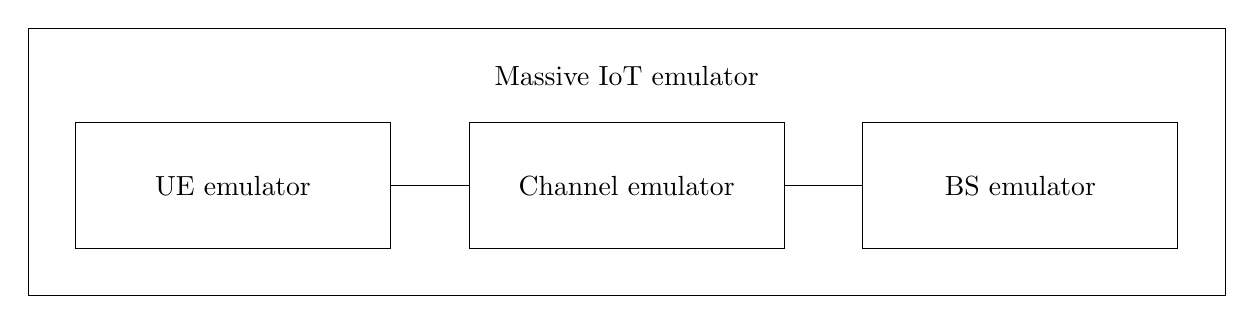
\begin{tikzpicture}[scale=0.2]

\draw  (-38,14) rectangle (38,-3);
\node at (0,11) {Massive IoT emulator};

\draw  (-35,8) rectangle (-15,0);
\node at (-25,4) {UE emulator};

\draw  (-10,8) rectangle (10,0);
\node at (0,4) {Channel emulator};

\draw  (35,8) rectangle (15,0);
\node at (25,4) {BS emulator};

\draw (-15,4) -- (-10,4);

\draw (10,4) -- (15,4);
\end{tikzpicture}}
%\caption{emulator overview}
%\label{fig:emulator_overview}
%\end{figure}
%
%The \gls{UEE} will be connected to the \gls{BSE} through a cable, this will remove the interference to and thereby the restriction of using licensed the licensed spectrum. This also means it would be advantageous to move the channel emulator to either the \gls{UEE} or the \gls{BSE}. 
%
%As mentioned in \autoref{ch:Introduction} the task is quite huge, therefore is it necessary to use existing software when possible and use experiences from earlier work in this field.
%
%
%\section{Earlier work}
%A similar system has been built before in 2017 by Mathias Kielgast and Anders Rasmussen \citep{thesis_report}. They used two \gls{SDR}s to emulate a basestation and multiple \gls{LTE} devices respectively. They took the existing srsUE system and changed the structure to handle multiple UEs. The design principle, as can also been seen in \autoref{fig:thesis_structure}, is to emulate multiple \gls{LTE} protocol stacks in which is connected to a commen physical layer. This allows for the multiple devices to be independent from each other, but still using the same \gls{SDR}. \citep{thesis_report} 
%
%\begin{figure}[H]
%\centering
%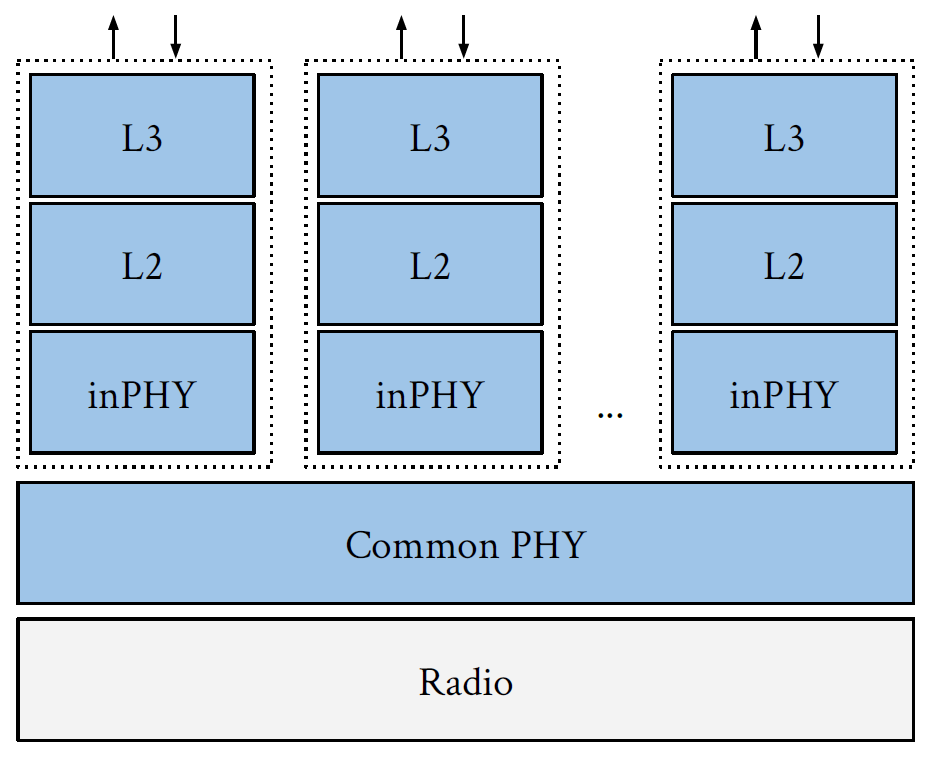
\includegraphics[width=0.7\textwidth]{figures/thesis_structure.png}
%\caption{thesis structure \citep{thesis_report}}
%\label{fig:thesis_structure}
%\end{figure}
%
%
%The system was made to prove if the method could work for a \gls{MTC} type of connection also. In this way they made a proof of concept product that emulated 15 devices using a 5 MHz bandwidth. They also proved that smaller bandwidth allowed the system to emulate more devices. The UEE used the the srsUE as a framework while the BSE used the \gls{OAI}. \citep{thesis_report} 
%
%The design of the \gls{MITE} relies heavily on the work done in this project. However as it is intended to use the \gls{NB-IoT} protocol instead of \gls{LTE} it is necessary to use another version of srsUE as well as another framework entirely for the \gls{BS} emulator. The \gls{BS} emulator will instead rely on the Amarisoft BSE.
%
%%\section{General Setup}
%\section{Basestation emulator}
%As found in the \autoref{ch:Introduction} there is two possibilities when choosing the \gls{BSE}, Amairsoft and SRS. It has been chosen to work with the Amarisoft \gls{BSE}, as it provides the necessary features and comes with support. The SRS \gls{BSE} is not yet fully developed so it might require a lot more time to get working. Another alternative altogether is the Keysight E7515A UXM, it also provides the needed features it is just a lot more expensive. Therefore the \gls{BSE} chosen is the Amarisoft LTE 100.
%
%Amarisoft LTE 100 features LTE, LTE-A, LTE-M and NB-IoT protocols.    For the NB-IoT protocol it specifically features\citep{Amarisoft_solutions}:
%
%\begin{itemize}
%\item NB-IoT release 14 compliant
%\item Single-tone and multi-tone category NB1 and NB2 UE support
%\item 15 kHz and 3.75 kHz subcarrier spacing are supported
%\item All operation modes (in-band, guard band and standalone) are supported
%\item Multiple NB-IoT and LTE cells can be used at the same time in the same eNodeB
%\item Support of multiple coverage levels
%\item Support of all NPDCCH, NPDSCH, NPUSCH and NPRACH configurations
%\item Support of control plane CIoT optimization
%\item Support of multi-DRB mode
%\end{itemize}
%
%\section{User Equipment Emulator}
%\subsection{Quectel}
%\subsection{SRS UE}
%
%
% and the channel emulator will be implemented only as a simple \gls{PL} factor. 
As seen for the description of the different components in the system, the chosen components for the massiveness and battery life part is different in multiple parts. An deeper inspection of the different setup for the two different parts will now been looked into.

\chapter{Battery life system overview}
\chapter{Massive IoT system overview}
\label{ch:MassOver}
The focus of this chapter is to provide an overview over the concepts and design of the \gls{MDE}. From \autoref{ch:NB-IoT} it is known that \todo{Insert knowledge fact about massive.} and a known concept is known from the project \citep{thesis_report}.

%It has a high cost to test massiveness scenarios with a massive amount of hardware devices and will require a system to control them individually, especially if the desire is to test the impact of massiveness on the individual devices. A more optimal solution is instead of buying a massive amount of devices, to emulate them through software.

To test the scenario of massiveness can be done in two ways, with a massive amount of hardware devices that require a system to control them individually or to emulate multiple devices in software using a minimal amount of hardware. For this type of emulation the optimal solution is the latter, as the desired amount of devices numbers several thousands. 
\todo{I like this way of describing it better what do you think?}

The challenges with emulating a massive amount of devices, is that every single device is complex, as seen through \autoref{ch:NB-IoT}, and not easy to emulate, as all the aspects of the devices functionalities are also wanted in the emulator. So to emulate a massive amount of devices, takes a lot of CPU power and memory to process the data for each individual device and containing the devices them self \todo{containing the devices them self???? what do you mean?}. Another challenge is that the signals have to be combined for the different devices and send to the eNB and the signal from the eNB have to be split up to all the devices and this have to be handled quickly as the system operate in real time.

As seen from \todo{Insert tabel ref from ch 2} there is multiple version of emulators for a single NB-IoT device, but as the protocol still is in development, these emulators are also in the development stage and they only emulate a single device. But as a foundation for the project the SRS NB-IoT emulator will be used as a baseline, as designing the emulator from scratch is undesired \todo{Find a good formulation here, happy?}. The SRS emulator is chosen, as it was accessible to get with the source code, as there have to be some restructure in the code, and it is based on the LTE emulator from SRS, which was used in \todo{CM ref}, were the base concept in this project will be taken from. \todo{this sentence is a mess, PS charlie's og mathias's report is }
%citep{thesis_report}
The SRS NB-IoT emulator is a bigger c++ code project structured up into classes. As the code was never intended to emulate multiple devices, several changes is needed, to emulate multiple devices.


%The concept to produce this type of emulator, with the focus on having as high a number of devices active, while they still keep all functionalities for the individual device, will be to split up the code up into common parts, which can be used for all devices, and individual parts, which are only used for the individual device. To make this split between parts, the baseline code will be investigated.

The key idea for the emulator, is to split between active and inactive devices. This is done to achieve as high a number of devices as possible. Each device needs to keep all functionalities of a device, however some functionalities should be common for all devices. These functionalities refers to the radio layer functionalities, as only one radio is used for all devices it makes sense to only handle the radio functionalities once and share the data later to each device. To do this the code should be split up into common parts, which can be used for all devices, and individual parts, which are only used for the individual device. To make this split between parts, the baseline code will be investigated.

\todo{Insert overall structure}
\todo{you have only explained the massive part of your emulator what about the rest?}
\todo{the idea german explained was to keep it in concept form first but not single out the emulator like this}





%For the emulation of the eNB the Amarisoft LTE 100 code will be used as it can handle 1000 \gls{UE}s \citep{Amarisoft_solutions} and is tested to synchronize with the software based NB-IoT devices that will be used. As it is a commercial BSE, it is not open source and therefore harder to add new features and change all parameters, but as the focus is the devices, the software will still be used. A longer list of parameters for the Amarisoft LTE 100 code can be found in \appref{app:Amarisoft}.

%For the \gls{MDE} the code from SRS which have been tested to work with the software eNB from Amarisoft is chosen. This is chosen primarily because access to the source code is available through Keysight Technologies. As the code is designed for a single device some change have to be implemented, which requires knowledge of the original code. 

%The code will produce the infrastructure of the \gls{MDE} combining and transmitting the signals produced to the \gls{eNB}. The eNB will be emulated on secondary PC, as this frees up the PC running the \gls{MDE}. The NB-IoT spectrum overlaps with the LTE or GSM spectrum, meaning the spectrum is licensed, therefore a wire is used to connect \gls{MDE} and eNB. As the path loss in the wire is quite low, compared to transmission through the air, a 30 dB attenuator is added in between to increase the dynamic spectrum of the \gls{MDE} and eNB. To convert from digital signals to RF signals, a USRP B210 is connected to each the two emulators as these \gls{SDR}s are comparable with both softwares. The setup of the emulators can be seen on \autoref{fig:MassSetup}.

%\tikzsetnextfilename{MassSetup}
%\begin{figure}[H]
%\centering
%\resizebox{0.9\textwidth}{!}{
%\input{figures/Mass_setup.tex}}
%\caption{Overview of the emulator setup}
%\label{fig:MassSetup}
%\end{figure}



%The emulation of the massiveness scenarios uses the Massive IoT and eNB (Amarisoft) components. It is possible to connect and external NB-IoT device be combining its signal with the signals from the other two components. But as the focus for this part of the emulator is to stress test the protocol this feature will not be used. The Orchestrator is not used either in this part, as it has not been prioritized to set the two system together and have the same control unit. Both components is started up from a config file. While the Amarisoft software already fits to the purpose as an eNB, the SRS software code need to be change to emulate multiple UE. To understand this changes, there will be looked into the original code

%\section{eNB emulator}
%For the emulation of the eNB the Amarisoft LTE 100 code will be used as it can handle 1000 \gls{UE} \todo{Insert ref to Amarisoft side} and is tested to synchronize with the software based NB-IoT devices that will be used. As it is a commercial BSE, it is not open source and therefore harder to add new features and change all parameters, but as the focus is the devices, the software will still be used. A longer list of parameters for the Amarisoft LTE 100 code can be found \todo{Insert appendix for this}

%\section{Massive device emulator}
%For the emulation of the massive amount of NB-IoT devices the code provide by SRS which have been tested to work with the software eNB from Amarisoft. As the code is design for a single device some change have to be implemented, which requires knowledge of the original code.



\section{Baseline emulator}
As stated before, is the baseline emulator from SRS stil in development. The structure of the code have been copied from the LTE version, where it follows the communication layer structure known from \autoref{ch:NB-IoT}. The code process only goes up to msg2, as SRS have not developed the functionalities to transmit msg3 correctly. This blocks the possibilities to make a full attach and transmit data and all other functionalities after completing an attach. But as a prove of concept, to showcase the possibility of emulating a massive amount of device, as this aspect is one of the new aspects that have to be taken into account when using NB-IoT.

%The code provide by SRS is still in development and is based on the code SRS developed to LTE, which was used in \citep{thesis_report}. The structure of the code is very similar and with that, some of the structure change and solutions can be copied over from the mentioned project.

%Unfortunately as the code is still in development, the msg3 transmission does not work, as it seems that it gets transmitted in a wrong time slot. \todo{Check up on if this is what we want to say} This block the possibility to get a complete attach request, so the project will only work up to the reception of msg2. The plans for the changes and solution for the parts including the full attach procedure and data transmission, can be found in \autoref{ch:Future}.

\subsection{Structure}
\label{sub:MassStruct}
To estimate the parts of the code that should be common for all devices  and which shall be kept individual, there is a need to understand the structure of the code and how it performs different part of the NB-IoT protocol. As stated before is that code is split up into multiple classes and it is structure much similar to the LTE version of the code and it follows the communication layer structure. Their is two part of the code which is the srsLTE, where all lower layer functionalities and the API to communicated

%The code is written in C++, with a little C in some of the lower level files. The code is divided up into two sections srsLTE, which contains all the lower layer functions and the radio layer, and srsUE, which emulate a device with all the different communication layers that handles the protocol. The code contains an amount of classes for the different layers known from the OSI model, as seen in \autoref{fig:MassClass}, with the PHY layer being split up into even more classes. All these classes is underclasses for an overall class called ue, which therefore contains all the parts needed for running a device.The structure of the PHY layer can be seen in \autoref{fig:PhyClass}. As multiple tasks is needed to be handled at the same time in the different layers, threading is used in multiple classes (PHY, PHCH recv, PHCH workers, MAC, RRC, GW).

\tikzsetnextfilename{MassClass}
\begin{figure}[H]
\centering
\resizebox{0.5\textwidth}{!}{
\usetikzlibrary{arrows}
\begin{tikzpicture}

\draw  (-3,1) rectangle (2,0);
\draw  (-3,1.5) rectangle (2,2.5);
\draw  (-3,3) rectangle (2,4);
\draw  (-3,4.5) rectangle (2,5.5);
\node at (-0.5,0.5) {Radio};
\node at (-0.5,2) {PHY};
\node at (-0.5,3.5) {MAC};
\node at (-0.5,5) {RLC};
\draw  (-3,6) rectangle (2,7);
\draw  (-5,7.5) rectangle (-1,8.5);
\node at (-0.5,6.5) {PDCP};
\node at (-3,8) {RRC};
\draw  (0,7.5) rectangle (2,8.5);
\node at (1,8) {GW};
\draw  (-5,10.5) rectangle (-1,11.5);
\draw  (-3,10) rectangle (2,9);
\node at (-3,11) {USIM};
\node at (-0.5,9.5) {NAS};

\draw [-triangle 60](-1,1) -- (-1,1.5);
\draw [-triangle 60](0,1.5) -- (0,1);
\draw [-triangle 60](-1,2.5) -- (-1,3);
\draw [-triangle 60](0,3) -- (0,2.5);
\draw [-triangle 60](-1,4) -- (-1,4.5);
\draw [-triangle 60](0,4.5) -- (0,4);
\draw [-triangle 60](-1,5.5) -- (-1,6);
\draw [-triangle 60](0,6) -- (0,5.5);
\draw [-triangle 60](-2.5,7) -- (-2.5,7.5);
\draw [-triangle 60](-1.5,7.5) -- (-1.5,7);
\draw [-triangle 60](0.5,7) -- (0.5,7.5);
\draw [-triangle 60](1.5,7.5) -- (1.5,7);
\draw [-triangle 60](0.5,8.5) -- (0.5,9);
\draw [-triangle 60](1.5,9) -- (1.5,8.5);
\draw [-triangle 60](-3,0.25) -- (-4.5,0.25) -- (-4.5,7.5);
\draw (-3,1.75) -- (-4.5,1.75);
\draw (-3,3.25) -- (-4.5,3.25);
\draw (-3,4.75) -- (-4.5,4.75);
\draw [-triangle 60](-3.5,7.5) -- (-3.5,5.25)  -- (-3,5.25);
\draw [-triangle 60](-3.5,7.5) -- (-3.5,3.75)  -- (-3,3.75);
\draw [-triangle 60](-3.5,7.5) -- (-3.5,2.25)  -- (-3,2.25);
\draw [-triangle 60](-3.5,7.5) -- (-3.5,0.75) -- (-3,0.75);
\draw [-triangle 60](-4.5,8.5) -- (-4.5,10.5);
\draw [-triangle 60](-3.5,10.5) -- (-3.5,8.5);
\draw [-triangle 60](-2.5,8.5) -- (-2.5,9);
\draw [-triangle 60](-1.5,9) -- (-1.5,8.5);
\draw [-triangle 60](-2.5,10) -- (-2.5,10.5);
\draw [-triangle 60](-1.5,10.5) -- (-1.5,10);
\end{tikzpicture}}
\caption{Class overview of SRS emulation code}
\label{fig:MassClass}
\end{figure}

\begin{figure}[H]
\centering
\tikzsetnextfilename{PhyClass}
\resizebox{0.5\textwidth}{!}{
\usetikzlibrary{arrows}
\begin{tikzpicture}

\draw  (-2.5,-1) rectangle (1.5,-3);
\draw  (-3,0) rectangle (2,-3.5);
\draw  (-7.5,-1) rectangle (-3.5,-3);
\draw  (-7.5,2.5) rectangle (2,0.5);
\draw  (-2.5,5) rectangle (1.5,3);
\node at (-1.75,-0.30) {Thread pool};
\node at (-0.5,-2) {PHCH workers};
\node at (-5.5,-2) {PHCH common};
\node at (-3.25,1.5) {PHCH recv};
\node at (-0.5,4) {NPRACH};
\draw [-triangle 60](-2.5,-2) -- (-3.5,-2);
\draw [-triangle 60](-7.5,1) -- (-8.5,1) -- (-8.5,-4.5);
\draw (-7.5,-2.5) -- (-8.5,-2.5);
\node at (-8.5,-4.75) {Radio};
\draw [-triangle 60](-0.5,0.5) -- (-0.5,0);
\draw [-triangle 60](-7.5,-1.5) -- (-8,-1.5)  -- (-8,5.5);
\draw (-7.5,2) -- (-8,2);
\node at (-8,5.75) {MAC};
\draw (-0.5,-3) -- (-0.5,-4) -- (-8,-4) -- (-8,-0);
\draw [-triangle 60](-0.5,2.5) -- (-0.5,3);
\draw [-triangle 60](-5.5,0.5) -- (-5.5,-1);
\draw [-triangle 60](-5.5,2.5) -- (-5.5,5.5);
\node at (-5.5,5.75) {RRC};
\draw (-2.5,4) -- (-8.5,4) -- (-8.5,0);
\end{tikzpicture}}
\caption{Class overview of the PHY layer from the SRS emulation code}
\label{fig:PhyClass}
\end{figure}

Even if the class layout look like the OSI model but it does not follow it on point especially the lower layers (PHY and MAC). This comes from that many of the MAC layers task is moved to the PHY class and normally the PHY layer is made up of physical components and do the task, that the SDR performs. The RLC, PDCP, GW, NAS and USIM classes is not used much, as their functionality is for the process after the RAP or at least msg4 have been received. Therefore have they not been though much development in the SRS code. Here following is a description of the different classes and their functionality:

\begin{itemize}
\item [Radio] The radio controls and sets all the parameters for the transmission and receiving. It is the only class connected to the SDR API and sends the data to it for transmission and receives data from it too. 
\item [PHY] The PHY class handles the synchronization, the receiving and decoding of MIB and SIBs messages and decoding and encoding of transmission and received data. As it have a high number of task, it is split up into an amount of underclasses.
	\begin{itemize}
	\item [PHCH recv] Controls the whole PHY class system. Keeps track on which state the system is in and activates the different underclasses in the PHY class.
	\item [PHCH common] Contains most parameters for the PHY underclasses, here under the RNTI's and metrics for UL and DL, and communication up to the MAC class and sends transmission data to the radio class.
	\item [PHCH workers] Handles all processing of data after decoding of MIB and SIBs messages, both encoding and decoding dependably on the grants granted by the MAC class. Their can be multiple workers for one device, but in these cases, their will only be used one.
	\item [Thread pool] Contains and controls the array of PHCH workers.	
	\item [NPRACH] Used to send msg1 in the RAP and keep track of the parameters set for this transmission, like preamble id.
	\end{itemize}
\item [MAC] Keep track of TTI and give grants to PHY class to decode and encode of DL and UL. Control flow from the PHY class to the RLC class. Take over the RAP from the NPRACH class for msg2 and onward.
%\item [RLC] Control data package sizes down to the MAC layer though a buffer, but this 
%\item [PDCP]
\item [RRC] Is the overall control class for the whole device. Here it control how far through the process the device is and if it got all the needed parameters, which is the reason for it being connected to all lower classes, besides the radio class.
%\item [GW]
%\item [NAS]
%\item [USIM]
\end{itemize}

Between these classes are there some interfaces, that handles the movement of data, grants, parameters and other information. These interfaces is build as a class for it self for each interface, with an overall interface for functionalities used multiple places.

\subsection{Execution of the code}
The code is build up into multiple section which runs at different times, which is shown in \autoref{fig:MassStep}. After the initialization, the steps is matching the steps needed for a device to connect to an eNB. The different threads will go to different state, depending on which step in the process the code have made it to.

\begin{figure}[H]
\centering
\tikzsetnextfilename{MassStep}
\resizebox{0.5\textwidth}{!}{
\usetikzlibrary{arrows}
\begin{tikzpicture}

\draw  (-5,5) rectangle (-2,3);
\draw  (-5,2.5) rectangle (-2,0.5);
\draw  (-1,2.5) rectangle (2,0.5);
\draw  (-1,0) rectangle (2,-2);
\draw  (-5,0) rectangle (-2,-2);
\draw  (-5,-2.5) rectangle (-2,-4.5);
\draw  (-1,-2.5) rectangle (2,-4.5);
\node at (-3.5,4) {Initialization};
\node at (-3.5,1.5) {Synchronization};
\node at (0.5,1.5) {MIB};
\node at (-3.5,-1) {SIB2};
\node at (0.5,-1) {SIB1};
\node at (-3.5,-3.5) {NPRACH};
\node at (0.5,-3.5) {RAP};
\draw [-triangle 60](-3.5,3) -- (-3.5,2.5);
\draw [-triangle 60](-2,1.5) -- (-1,1.5);
\draw [-triangle 60](0.5,0.5) -- (0.5,0);
\draw [-triangle 60](-1,-1) -- (-2,-1);
\draw [-triangle 60](-3.5,-2) -- (-3.5,-2.5);
\draw [-triangle 60](-2,-3.5) -- (-1,-3.5);
\end{tikzpicture}}
\caption{A simplification of the steps in the code process}
\label{fig:MassStep}
\end{figure}

\textbf{Initialization} \\
The initialization step starts up all the different classes and sets pointers to the different interfaces between them and read the config file, which includes a longer list of parameters, which can be found in \appref{app:SRSconfig}. The PHY have a number of underclasses and which are initialized in the PHY thread, which close down afterwards. The main thread will wait on the PHY to finish initialize, before sending an attach request, through the NAS class. This process is shown in \autoref{fig:InitStep}.

\begin{figure}[H]
\centering
\tikzsetnextfilename{InitStep}
\resizebox{0.5\textwidth}{!}{
\usetikzlibrary{arrows}
\begin{tikzpicture}


\draw  (-4,3) rectangle (-1,1.5);
\draw  (-8,3) rectangle (-5,1.5);
\draw  (-8,1) rectangle (-5,-0.5);
\draw  (-8,-1) rectangle (-5,-2.5);
\draw  (-8,-3) rectangle (-5,-4.5);
\draw  (-3.5,-1) rectangle (-0.5,-2.5);
\draw  (-3.5,-3) rectangle (-0.5,-4.5);
\draw  (-8,-5) rectangle (-5,-6.5);
\draw  (-4,-0.5) rectangle (0,-5);

\draw [-triangle 90](-4,2.25) -- (-5,2.25);
\draw [-triangle 90](-6.5,1.5) -- (-6.5,1);
\draw [-triangle 90](-6.5,-0.5) -- (-6.5,-1);
\draw [-triangle 90](-6.5,-2.5) -- (-6.5,-3);
\draw [-triangle 90](-6.5,-4.5) -- (-6.5,-5);
\draw [dash pattern=on 2pt off 3pt on 4pt off 4pt][-triangle 90](-5,0.25) -- (-2,0.25) -- (-2,-1);
\draw [dash pattern=on 2pt off 3pt on 4pt off 4pt][-triangle 90](-2,-4.5) -- (-2,-5.75) -- (-5,-5.75);
\draw [-triangle 90](-2,-2.5) -- (-2,-3);

\node at (-2.5,2.25) {Start};
\node at (-6.5,2.25) {Read config file};
\node at (-6.5,0.25) {Start PHY init};
\node at (-6.5,-1.75) {Radio init};
\node at (-6.5,-3.75) {Upper layers init};
\node at (-6.5,-5.75) {Wait for PHY};
\node at (-2,-1.75) {Underclasses init};
\node at (-2,-3.75) {PHCH recv init};
\draw [-triangle 60](-6.5,-6.5) -- (-6.5,-7.5);
\node at (-6.5,-7.75) {Attach request};
\node at (-0.50,-0.25) {PHY};
\end{tikzpicture}}
\caption{The process for the initialization. The dashed line indicates a event trigger to another thread.}
\label{fig:InitStep}
\end{figure}


\textbf{Synchronization and MIB} \\
The synchronization is where the device tries to find the NPSS and NSSS in the right frequency. This is done in the PHCH recv class, which handles both the synchronization and MIB, which is also decode here. The PHCH recv main functionalities is triggered in the loop, which run in it threads. This functionalities is triggered dependably on which state the class is in, which is shown in \autoref{fig:RecvState}.

\begin{figure}[H]
\centering
\tikzsetnextfilename{RecvState}
\resizebox{0.5\textwidth}{!}{
\usetikzlibrary{arrows}
\begin{tikzpicture}

\draw  (-4.5,1.5) ellipse (2 and 1);
\draw  (-4.5,4.5) ellipse (2 and 1);
\draw  (-4.5,7.5) ellipse (2 and 1);
\draw  (-4.5,10.5) ellipse (2 and 1);
\draw  [ultra thick](-11,6) ellipse (2 and 1);
\draw [-triangle 90](-4.5,9.5) -- (-4.5,8.5);
\draw [-triangle 90](-4.5,6.5) -- (-4.5,5.5);
\draw [-triangle 90](-4.5,3.5) -- (-4.5,2.5);
\draw [-triangle 90](-11,7) -- (-11,12.5) -- (-4.5,12.5) -- (-4.5,11.5);
\draw [-triangle 90](-2.75,8) -- (0,8) -- (0,10.5) -- (-2.5,10.5);
\draw [-triangle 90](-6.5,10.5) -- (-7.5,10.5) -- (-7.5,6) node (v1) {} -- (-9,6);
\draw [-triangle 90](-2.75,7) -- (0,7) -- (0,1.5) -- (-2.5,1.5);
\draw (-6.5,7.5) -- (-7.5,7.5);
\draw (-6.5,1.5) -- (-7.5,1.5) -- (-7.5,8.5);
\node at (-11,6) {Ilde};
\node at (-4.5,10.5) {Cell search};
\node at (-4.5,7.5) {Cell select};
\node at (-4.5,4.5) {Cell measure};
\node at (-4.5,1.5) {Cell camp};
\draw (-6.5,4.5) -- (-7.5,4.5);
\node at (-12,8) {Start sync};
\draw  (v1) ellipse (0.5 and 5.5);
\node at (-7.5,0) {Error or};
\node at (-7.5,-0.5) {Reset};
\node at (-3,9.25) {NPSS and NSSS};
\node at (-3,8.75) {found};
\node at (1.5,9.5) {Can not find};
\node at (1.5,9) {MIB};
\node at (2,4.75) {RSRP measurement};
\node at (2,4.25) {already done};
\node at (-2.5,6) {RSRP measurement};
\node at (-2.5,3) {Measurement done};
\end{tikzpicture}}
\caption{State machine for PHCH recv. The whole process start in ilde.}
\label{fig:RecvState}
\end{figure}
\todo{Write triggers into diagram}

The PHCH recv is in idle, until it gets triggered by the attach request, which have gone from the NAS to the RRC to the PHY, which then call sync start, so the state becomes cell search.

In cell search, the PHCH recv starts up the radio class and begins to receive signals from it, where it looks for the NPSS and NSSS through all different frequencies, where it will chose the one with the highest peak, over a certain level. If it does not find a frequency, where there supposed to be a cell, it retries and are stuck in this loop. If it finds a cell, it will then try to locate the MIB from the information from NPSS and NSSS. If it is found, the change the state from cell search to cell select.

In cell select the MIB is received and decoded and send to the MAC. In the case that it is not received well and can not be decoded in the first try \todo{Insert part with soft combining}. If it gets decode it will jump to cell measure, if their is none rsrp measurements \todo{gls maybe} or directly jump to cell camp, where it will begin to look into the SIB messages.

In cell measure it will measure the rsrp to correct the receiving parameters and then change to the cell camp stage.

Cell camp is the PHCH recv stage, where all further process will be handle, which starts out with the locating the SIB messages.

From all stages can the process be triggered to go into idle state, if an error occurred or the system tries to reset. Here it will try to start up into cell search again unless if it is the close down trigger.

\textbf{SIB1 and SIB2} \\
When the PHCH recv is in cell camp state, is it ready to activate the PHCH workers.




















To have the code emulate multiple devices, some parts of the original device is needed to be duplicated. The goal of these changes will be to have a massive amount of individual devices emulated, without them effecting each other through their processing time and combining their signals and transmit it as one to the eNB.

\section{Changed code}

\textbf{Structure}\\
\textbf{Flow of the code}\\

\chapter{Testing of Massive IoT system} \label{ch:mass_test}
The focus of this chapter is to showcase the emulator describe in \autoref{ch:MassOver}. This is done in a series of test, where it is compared to the original code and to see if the changed made for fill the goal set in \autoref{ch:MassOver}:

\textit{The goal of these changes will be to have a massive amount of individual devices emulated, without them effecting each other through their processing time and combining their signals and transmit it as one to the eNB.}

This will be done by comparing the changed code to the baseline code as well as testing the performance of the code at higher number of devices emulated.
The performance criteria that will be look into is:

\begin{itemize}
\item CPU usage
\item Memory usage
\item Execution time
\item Error rate
\end{itemize}

CPU and memory usage is used to test where possible bottle necks can be compared to overloading the used computer. CPU usage will be measure with the CPU stat tool, which can measure the CPU usage on the individual kernels at a sample rate of 3 Hz. The memory usage is measured using the system monitor tool, as all bigger buffers is allocated in the initialization and the used memory therefore is nearly static. 

The execution time will be look into to see if any processes in code is taking longer, after the changes. This will be measured by inserting prints of time stamps into the code, when the code goes from one step to another. 

Lastly the error rate will showcase the stability of the code. This is done by running the code multiple times and to analyze the errors occurring. The errors can be analyzed from the log files, produce by the code, when executed.

The parameters used for the eNB and SRS code is the default settings shown in \todo{Insert app ref to the two apps}. The test will be split up into the different steps in the code process discussed in \autoref{sub:MassStruct}.

\section{Error rate}
The error rate is found by 20 trials at each number of devices, until the emulator hit 100\% in error rate. Beside testing the emulator with the changed code, the baseline code will also be tested, but as it can only emulate one devices, this will be what the code will be matched against. These result can be seen in \autoref{fig:MT_error}.

\begin{figure}[H]
\tikzsetnextfilename{MT_error}
\centering
\resizebox{0.5\textwidth}{!}{
% This file was created by matlab2tikz.
%
%The latest updates can be retrieved from
%  http://www.mathworks.com/matlabcentral/fileexchange/22022-matlab2tikz-matlab2tikz
%where you can also make suggestions and rate matlab2tikz.
%
\definecolor{mycolor1}{rgb}{0.00000,0.44700,0.74100}%
\definecolor{mycolor2}{rgb}{0.85000,0.32500,0.09800}%
%
\begin{tikzpicture}

\begin{axis}[%
width=4.521in,
height=3.566in,
at={(0.758in,0.481in)},
scale only axis,
xmin=1,
xmax=15,
xlabel={Number of UEs},
ymin=0,
ymax=100,
ylabel={Error rate (\%)},
axis background/.style={fill=white},
title style={font=\bfseries},
title={Error rate},
legend style={at={(0.03,0.97)},anchor=north west,legend cell align=left,align=left,draw=white!15!black}
]
\addplot [color=mycolor1,solid]
  table[row sep=crcr]{%
1	25\\
2	40\\
3	25\\
4	15\\
5	40\\
6	30\\
7	30\\
8	20\\
9	15\\
10	50\\
11	30\\
12	20\\
13	100\\
14	100\\
15	100\\
};
\addlegendentry{Change code};

\addplot [color=mycolor2,solid]
  table[row sep=crcr]
\caption{Error rate for different amount of devices.}
\label{fig:MT_error}
\end{figure}

As it can be seen in \autoref{fig:MT_error}, the error rate is higher for the changed code, than the baseline which still is not perfect. Another important aspect is that when the number of devices hit 13, the error rate goes to 100\%, which shows the limit of the emulator. To get a better understanding of these error, a diagram over the different error is shown in \autoref{fig:MT_error_dist}.

\begin{figure}[H]
\tikzsetnextfilename{MT_error_dist}
\centering
\resizebox{0.8\textwidth}{!}{
% This file was created by matlab2tikz.
%
%The latest updates can be retrieved from
%  http://www.mathworks.com/matlabcentral/fileexchange/22022-matlab2tikz-matlab2tikz
%where you can also make suggestions and rate matlab2tikz.
%
\definecolor{mycolor1}{rgb}{0.20810,0.16630,0.52920}%
\definecolor{mycolor2}{rgb}{0.01651,0.42660,0.87863}%
\definecolor{mycolor3}{rgb}{0.02650,0.61370,0.81350}%
\definecolor{mycolor4}{rgb}{0.21783,0.72504,0.61926}%
\definecolor{mycolor5}{rgb}{0.64730,0.74560,0.41880}%
\definecolor{mycolor6}{rgb}{0.99377,0.74546,0.24035}%
\definecolor{mycolor7}{rgb}{0.97630,0.98310,0.05380}%
%
\begin{tikzpicture}

\begin{axis}[%
width=.8\textwidth,
height=.533\textwidth,
at={(0.533in,0.481in)},
scale only axis,
bar width=0.5,
xmin=-0.5,
xmax=15.5,
xtick={0,1,2,3,4,5,6,7,8,9,10,11,12,13,14,15},
xticklabels={{Base},{1},{2},{3},{4},{5},{6},{7},{8},{9},{10},{11},{12},{13},{14},{15}},
xlabel={Number of devices},
ymin=0,
ymax=100,
ylabel={Trials},
axis background/.style={fill=white},
title style={font=\bfseries},
title={Error distrubution},
legend style={at={(1.03,1)},anchor=north west,legend cell align=left,align=left,draw=white!15!black}
]
\addplot[ybar stacked,draw=black,fill=mycolor1,area legend] plot table[row sep=crcr] {%
0	90\\
1	75\\
2	60\\
3	75\\
4	85\\
5	60\\
6	70\\
7	70\\
8	80\\
9	85\\
10	50\\
11	70\\
12	80\\
13	0\\
14	0\\
15	0\\
};
\addlegendentry{No errors};

\addplot[ybar stacked,draw=black,fill=mycolor2,area legend] plot table[row sep=crcr] {%
0	0\\
1	0\\
2	0\\
3	0\\
4	0\\
5	0\\
6	0\\
7	0\\
8	5\\
9	0\\
10	0\\
11	0\\
12	0\\
13	5\\
14	0\\
15	0\\
};
\addlegendentry{Cell sync error};

\addplot[ybar stacked,draw=black,fill=mycolor3,area legend] plot table[row sep=crcr] {%
0	10\\
1	10\\
2	10\\
3	10\\
4	0\\
5	15\\
6	15\\
7	5\\
8	10\\
9	5\\
10	15\\
11	15\\
12	10\\
13	0\\
14	15\\
15	5\\
};
\addlegendentry{Radio error};

\addplot[ybar stacked,draw=black,fill=mycolor4,area legend] plot table[row sep=crcr] {%
0	0\\
1	10\\
2	30\\
3	15\\
4	15\\
5	25\\
6	10\\
7	25\\
8	5\\
9	5\\
10	30\\
11	5\\
12	5\\
13	80\\
14	65\\
15	60\\
};
\addlegendentry{Idle after MIB-NB};

\addplot[ybar stacked,draw=black,fill=mycolor5,area legend] plot table[row sep=crcr] {%
0	0\\
1	0\\
2	0\\
3	0\\
4	0\\
5	0\\
6	0\\
7	0\\
8	0\\
9	5\\
10	5\\
11	10\\
12	5\\
13	5\\
14	10\\
15	20\\
};
\addlegendentry{Transmission after NB-SIB1};

\addplot[ybar stacked,draw=black,fill=mycolor6,area legend] plot table[row sep=crcr] {%
0	0\\
1	0\\
2	0\\
3	0\\
4	0\\
5	0\\
6	5\\
7	0\\
8	0\\
9	0\\
10	0\\
11	0\\
12	0\\
13	10\\
14	10\\
15	10\\
};
\addlegendentry{NPRACH error};

\addplot[ybar stacked,draw=black,fill=mycolor7,area legend] plot table[row sep=crcr] 
\caption{The distribution of different errors for different amount of devices.}
\label{fig:MT_error_dist}
\end{figure}

As seen in \autoref{fig:MT_error_dist} is there six different types of errors that have occurred in the testing.

Radio error is the only error type that the baseline also have. It comes from miscommunication between the radio class and the API for the USRP B210. It occur when the process begins the search after SIB messages, where some radio parameters is changed. As the radio error is the only error occurring for the baseline, this should be the only error which are not produced by the changed made to the baseline.

The ilde after MIB error occur in the same part of the process as the radio error, where the emulator gets stuck and runs without retrying or closing down. This error type is the most occurring type of the errors produced by the changes, which will be the most optimal place to improve the error rate, especially for higher amount of devices.

The msg2 not received error is when all devices have gone through the NPRACH step and waiting on the msg2, which is never received or not registered if received. This error is very rare and have no tendencies.

Cell sync error is when the emulator shuts down before a synchronization is finalized and it goes to the MIB step. This errors is very rare, but as the error occurs so early in the process, these test runs will not give any data for any other step, beside initialization.

Transmission after SIB1 is an error that occurs sometimes at the SIB1 step and the radio class transmit a signal, which course the emulator to shut down. This error type have a tendency to occur with higher amount of devices and can indicate a bottleneck in the process to get a higher amount of devices.

NPRACH error is an error that occurs when some devices completes the NPRACH step, but other do not, as the system shuts down before hand. This error type have the same tendency as the transmission after SIB1 error and indicates the same thing.





\section{Initialization}

\begin{figure}[H]
\tikzsetnextfilename{MT_Init_Time}
\centering
\resizebox{0.5\textwidth}{!}{
% This file was created by matlab2tikz.
%
%The latest updates can be retrieved from
%  http://www.mathworks.com/matlabcentral/fileexchange/22022-matlab2tikz-matlab2tikz
%where you can also make suggestions and rate matlab2tikz.
%
\definecolor{mycolor1}{rgb}{0.00000,0.44700,0.74100}%
\definecolor{mycolor2}{rgb}{0.85000,0.32500,0.09800}%
%
\begin{tikzpicture}

\begin{axis}[%
width=4.521in,
height=3.566in,
at={(0.758in,0.481in)},
scale only axis,
xmin=-0.5,
xmax=15.5,
xtick={0,1,2,3,4,5,6,7,8,9,10,11,12,13,14,15},
xticklabels={{Baseline},{1},{2},{3},{4},{5},{6},{7},{8},{9},{10},{11},{12},{13},{14},{15}},
xlabel={Number of UEs},
ymin=1.4,
ymax=3.2,
ylabel={Time (s)},
axis background/.style={fill=white},
title style={font=\bfseries},
title={Initialization time},
legend style={at={(0.03,0.97)},anchor=north west,legend cell align=left,align=left,draw=white!15!black}
]
\addplot [color=mycolor1,only marks,mark=*,mark options={solid}]
  table[row sep=crcr]{%
1	1.60657000541687\\
1	1.60206508636475\\
1	1.60402417182922\\
1	1.60998201370239\\
1	1.59828901290894\\
1	1.59890818595886\\
1	1.60678696632385\\
1	1.70481204986572\\
1	1.60345387458801\\
1	1.59799599647522\\
1	1.60137987136841\\
1	1.60408782958984\\
1	1.60380721092224\\
1	1.61764979362488\\
1	1.61315512657166\\
1	1.60408186912537\\
1	1.60214781761169\\
1	1.59820103645325\\
1	1.70323586463928\\
1	1.60239100456238\\
};
\addlegendentry{Change code};

\addplot [color=mycolor1,only marks,mark=*,mark options={solid}]
  table[row sep=crcr]{%
2	1.70376014709473\\
2	1.69752597808838\\
2	1.69991588592529\\
2	1.70224094390869\\
2	1.70335793495178\\
2	1.70019602775574\\
2	1.81223583221436\\
2	1.70259284973145\\
2	1.70058512687683\\
2	1.90431618690491\\
2	1.69746613502502\\
2	1.70056891441345\\
2	1.7057900428772\\
2	1.6926589012146\\
2	1.69660997390747\\
2	1.69284415245056\\
2	1.70735216140747\\
2	1.69585204124451\\
2	1.69405889511108\\
2	1.70744895935059\\
};
\addlegendentry{Baseline};

\addplot [color=mycolor1,only marks,mark=*,mark options={solid}]
  table[row sep=crcr]{%
3	1.79403805732727\\
3	1.80174088478088\\
3	1.80632400512695\\
3	1.79517197608948\\
3	1.7999119758606\\
3	1.80256199836731\\
3	1.79768395423889\\
3	1.79976677894592\\
3	1.79294800758362\\
3	1.80160784721375\\
3	1.81014108657837\\
3	1.8038489818573\\
3	1.79714298248291\\
3	1.78692388534546\\
3	1.80100011825562\\
3	1.79488515853882\\
3	1.81216788291931\\
3	1.79761385917664\\
3	1.80774402618408\\
3	1.79226994514465\\
};
\addlegendentry{Fitted line};

\addplot [color=mycolor1,only marks,mark=*,mark options={solid},forget plot]
  table[row sep=crcr]{%
4	1.98840284347534\\
4	1.98891401290894\\
4	1.90781497955322\\
4	1.90410208702087\\
4	1.89322519302368\\
4	1.89481401443481\\
4	1.89260292053223\\
4	1.89337205886841\\
4	1.89051008224487\\
4	1.99312591552734\\
4	1.89608120918274\\
4	1.98998594284058\\
4	1.9188380241394\\
4	1.88647603988647\\
4	1.89477205276489\\
4	1.89825892448425\\
4	1.90163683891296\\
4	1.89038610458374\\
4	1.91325998306274\\
4	1.88523697853088\\
};
\addplot [color=mycolor1,only marks,mark=*,mark options={solid},forget plot]
  table[row sep=crcr]{%
5	1.99140405654907\\
5	1.98323607444763\\
5	2.10928916931152\\
5	1.97859597206116\\
5	2.08593010902405\\
5	1.97863793373108\\
5	1.99062418937683\\
5	2.07845187187195\\
5	1.99165511131287\\
5	1.97789597511292\\
5	1.98802804946899\\
5	1.9954240322113\\
5	2.00401997566223\\
5	1.98706889152527\\
5	1.98496317863464\\
5	1.97689509391785\\
5	1.98235487937927\\
5	1.98183512687683\\
5	2.10645198822021\\
5	1.97618389129639\\
};
\addplot [color=mycolor1,only marks,mark=*,mark options={solid},forget plot]
  table[row sep=crcr]{%
6	2.07043600082397\\
6	2.08795213699341\\
6	2.08343291282654\\
6	2.09298491477966\\
6	2.07702803611755\\
6	2.07426118850708\\
6	2.1002459526062\\
6	2.09029412269592\\
6	2.08507609367371\\
6	2.07489895820618\\
6	2.08115887641907\\
6	2.09077501296997\\
6	2.08771395683289\\
6	2.07395005226135\\
6	2.07281303405762\\
6	2.1818699836731\\
6	2.08554911613464\\
6	2.0755889415741\\
6	2.09108996391296\\
6	2.08529710769653\\
};
\addplot [color=mycolor1,only marks,mark=*,mark options={solid},forget plot]
  table[row sep=crcr]{%
7	2.16757988929749\\
7	2.16262793540955\\
7	2.17564296722412\\
7	2.1759250164032\\
7	2.19155502319336\\
7	2.27151203155518\\
7	2.1676127910614\\
7	2.17567276954651\\
7	2.17186117172241\\
7	2.29317903518677\\
7	2.17238211631775\\
7	2.17540311813354\\
7	2.17659687995911\\
7	2.16815400123596\\
7	2.17439103126526\\
7	2.17733693122864\\
7	2.17026114463806\\
7	2.17389607429504\\
7	2.19961309432983\\
7	2.1946439743042\\
};
\addplot [color=mycolor1,only marks,mark=*,mark options={solid},forget plot]
  table[row sep=crcr]{%
8	2.27100706100464\\
8	2.26513481140137\\
8	2.26285195350647\\
8	2.2616548538208\\
8	2.27730703353882\\
8	2.27119493484497\\
8	2.26165103912354\\
8	2.25236415863037\\
8	2.26101899147034\\
8	2.36273288726807\\
8	2.25905799865723\\
8	2.27876305580139\\
8	2.29212021827698\\
8	2.26190590858459\\
8	2.27887606620789\\
8	2.25859999656677\\
8	2.26044893264771\\
8	2.26256895065308\\
8	2.26363897323608\\
8	2.26199913024902\\
};
\addplot [color=mycolor1,only marks,mark=*,mark options={solid},forget plot]
  table[row sep=crcr]{%
9	2.35985803604126\\
9	2.35758590698242\\
9	2.35490608215332\\
9	2.35805201530457\\
9	2.35813903808594\\
9	2.36619591712952\\
9	2.36291694641113\\
9	2.3615140914917\\
9	2.36494493484497\\
9	2.35645508766174\\
9	2.36352205276489\\
9	2.36592721939087\\
9	2.46607184410095\\
9	2.46248698234558\\
9	2.35874915122986\\
9	2.35979104042053\\
9	2.36403608322144\\
9	2.35437083244324\\
9	2.45976400375366\\
9	2.35649704933167\\
};
\addplot [color=mycolor1,only marks,mark=*,mark options={solid},forget plot]
  table[row sep=crcr]{%
10	2.4522500038147\\
10	2.45602107048035\\
10	2.45017790794373\\
10	2.46005892753601\\
10	2.4437301158905\\
10	2.45332884788513\\
10	2.45075607299805\\
10	2.44673299789429\\
10	2.44251298904419\\
10	2.45762705802917\\
10	2.45294904708862\\
10	2.48201680183411\\
10	2.45067620277405\\
10	2.57340097427368\\
10	2.44935178756714\\
10	2.45021200180054\\
10	2.55899405479431\\
10	2.55124402046204\\
10	2.45972394943237\\
10	2.4552149772644\\
};
\addplot [color=mycolor1,only marks,mark=*,mark options={solid},forget plot]
  table[row sep=crcr]{%
11	2.54409885406494\\
11	2.5580689907074\\
11	2.55131316184998\\
11	2.54538011550903\\
11	2.54991102218628\\
11	2.54586219787598\\
11	2.54519009590149\\
11	2.54685091972351\\
11	2.54958415031433\\
11	2.55115580558777\\
11	2.55340099334717\\
11	2.54899501800537\\
11	2.54859089851379\\
11	2.55042195320129\\
11	2.54939794540405\\
11	2.57132411003113\\
11	2.54307293891907\\
11	2.54036903381348\\
11	2.54952502250671\\
11	2.56598615646362\\
};
\addplot [color=mycolor1,only marks,mark=*,mark options={solid},forget plot]
  table[row sep=crcr]{%
12	2.63736891746521\\
12	2.6386501789093\\
12	2.63579487800598\\
12	2.76004385948181\\
12	2.64884686470032\\
12	2.63978505134583\\
12	2.65288496017456\\
12	2.6491858959198\\
12	2.64470791816711\\
12	2.65107917785645\\
12	2.83676886558533\\
12	2.63889098167419\\
12	2.65938687324524\\
12	2.6382257938385\\
12	2.63785290718079\\
12	2.65852999687195\\
12	2.74441695213318\\
12	2.64707398414612\\
12	2.63858604431152\\
12	2.65901207923889\\
};
\addplot [color=mycolor1,only marks,mark=*,mark options={solid},forget plot]
  table[row sep=crcr]{%
13	2.73925495147705\\
13	2.76844787597656\\
13	2.74468803405762\\
13	2.72794198989868\\
13	2.73288083076477\\
13	2.72759079933167\\
13	2.73981499671936\\
13	2.73808693885803\\
13	2.73037505149841\\
13	2.73060989379883\\
13	2.75299692153931\\
13	2.73150610923767\\
13	2.73392391204834\\
13	2.83988189697266\\
13	2.73668503761292\\
13	2.73319101333618\\
13	2.7269880771637\\
13	2.73366594314575\\
13	2.73546814918518\\
13	2.73145604133606\\
};
\addplot [color=mycolor1,only marks,mark=*,mark options={solid},forget plot]
  table[row sep=crcr]{%
14	2.93708896636963\\
14	2.8230938911438\\
14	2.82491183280945\\
14	2.81724190711975\\
14	2.83096098899841\\
14	2.82523608207703\\
14	2.92713284492493\\
14	2.83528399467468\\
14	2.81740093231201\\
14	2.94761514663696\\
14	2.84746098518372\\
14	2.92244791984558\\
14	2.82092189788818\\
14	2.82772517204285\\
14	2.82116103172302\\
14	2.8086531162262\\
14	2.82523202896118\\
14	2.82433700561523\\
14	2.85196495056152\\
14	2.82061409950256\\
};
\addplot [color=mycolor1,only marks,mark=*,mark options={solid},forget plot]
  table[row sep=crcr]{%
15	2.91355895996094\\
15	2.92956900596619\\
15	2.92799687385559\\
15	3.0291600227356\\
15	2.92018890380859\\
15	2.92904806137085\\
15	2.91579508781433\\
15	2.91569089889526\\
15	2.92359805107117\\
15	2.91793894767761\\
15	2.9355640411377\\
15	3.12653303146362\\
15	2.91362810134888\\
15	2.94397902488709\\
15	2.9135410785675\\
15	2.91744613647461\\
15	2.92062401771545\\
15	2.91158103942871\\
15	3.02637410163879\\
15	2.90584707260132\\
};
\addplot [color=mycolor2,only marks,mark=*,mark options={solid},forget plot]
  table[row sep=crcr]{%
0	1.51574110984802\\
0	1.60954785346985\\
0	1.61224007606506\\
0	1.51666712760925\\
0	1.51392078399658\\
0	1.51035499572754\\
0	1.50713300704956\\
0	1.51292109489441\\
0	1.51016092300415\\
0	1.5099790096283\\
0	1.51415991783142\\
0	1.51640319824219\\
0	1.51323890686035\\
0	1.51066589355469\\
0	1.5165901184082\\
0	1.50853300094604\\
0	1.50311899185181\\
0	1.60737919807434\\
0	1.51729917526245\\
0	1.50886988639832\\
};
\addplot [color=red,solid,forget plot]
  table[row sep=crcr]{%
0	1.52591009015129\\
0.015	1.52732309482467\\
0.03	1.52873609949805\\
0.045	1.53014910417142\\
0.06	1.5315621088448\\
0.075	1.53297511351818\\
0.09	1.53438811819156\\
0.105	1.53580112286494\\
0.12	1.53721412753832\\
0.135	1.5386271322117\\
0.15	1.54004013688508\\
0.165	1.54145314155845\\
0.18	1.54286614623183\\
0.195	1.54427915090521\\
0.21	1.54569215557859\\
0.225	1.54710516025197\\
0.24	1.54851816492535\\
0.255	1.54993116959873\\
0.27	1.55134417427211\\
0.285	1.55275717894549\\
0.3	1.55417018361886\\
0.315	1.55558318829224\\
0.33	1.55699619296562\\
0.345	1.558409197639\\
0.36	1.55982220231238\\
0.375	1.56123520698576\\
0.39	1.56264821165914\\
0.405	1.56406121633252\\
0.42	1.56547422100589\\
0.435	1.56688722567927\\
0.45	1.56830023035265\\
0.465	1.56971323502603\\
0.48	1.57112623969941\\
0.495	1.57253924437279\\
0.51	1.57395224904617\\
0.525	1.57536525371955\\
0.54	1.57677825839293\\
0.555	1.5781912630663\\
0.57	1.57960426773968\\
0.585	1.58101727241306\\
0.6	1.58243027708644\\
0.615	1.58384328175982\\
0.63	1.5852562864332\\
0.645	1.58666929110658\\
0.66	1.58808229577996\\
0.675	1.58949530045333\\
0.69	1.59090830512671\\
0.705	1.59232130980009\\
0.72	1.59373431447347\\
0.735	1.59514731914685\\
0.75	1.59656032382023\\
0.765	1.59797332849361\\
0.78	1.59938633316699\\
0.795	1.60079933784036\\
0.81	1.60221234251374\\
0.825	1.60362534718712\\
0.84	1.6050383518605\\
0.855	1.60645135653388\\
0.87	1.60786436120726\\
0.885	1.60927736588064\\
0.9	1.61069037055402\\
0.915	1.6121033752274\\
0.93	1.61351637990077\\
0.945	1.61492938457415\\
0.96	1.61634238924753\\
0.975	1.61775539392091\\
0.99	1.61916839859429\\
1.005	1.62058140326767\\
1.02	1.62199440794105\\
1.035	1.62340741261443\\
1.05	1.6248204172878\\
1.065	1.62623342196118\\
1.08	1.62764642663456\\
1.095	1.62905943130794\\
1.11	1.63047243598132\\
1.125	1.6318854406547\\
1.14	1.63329844532808\\
1.155	1.63471145000146\\
1.17	1.63612445467484\\
1.185	1.63753745934821\\
1.2	1.63895046402159\\
1.215	1.64036346869497\\
1.23	1.64177647336835\\
1.245	1.64318947804173\\
1.26	1.64460248271511\\
1.275	1.64601548738849\\
1.29	1.64742849206187\\
1.305	1.64884149673524\\
1.32	1.65025450140862\\
1.335	1.651667506082\\
1.35	1.65308051075538\\
1.365	1.65449351542876\\
1.38	1.65590652010214\\
1.395	1.65731952477552\\
1.41	1.6587325294489\\
1.425	1.66014553412227\\
1.44	1.66155853879565\\
1.455	1.66297154346903\\
1.47	1.66438454814241\\
1.485	1.66579755281579\\
1.5	1.66721055748917\\
1.515	1.66862356216255\\
1.53	1.67003656683593\\
1.545	1.67144957150931\\
1.56	1.67286257618268\\
1.575	1.67427558085606\\
1.59	1.67568858552944\\
1.605	1.67710159020282\\
1.62	1.6785145948762\\
1.635	1.67992759954958\\
1.65	1.68134060422296\\
1.665	1.68275360889634\\
1.68	1.68416661356971\\
1.695	1.68557961824309\\
1.71	1.68699262291647\\
1.725	1.68840562758985\\
1.74	1.68981863226323\\
1.755	1.69123163693661\\
1.77	1.69264464160999\\
1.785	1.69405764628337\\
1.8	1.69547065095674\\
1.815	1.69688365563012\\
1.83	1.6982966603035\\
1.845	1.69970966497688\\
1.86	1.70112266965026\\
1.875	1.70253567432364\\
1.89	1.70394867899702\\
1.905	1.7053616836704\\
1.92	1.70677468834378\\
1.935	1.70818769301715\\
1.95	1.70960069769053\\
1.965	1.71101370236391\\
1.98	1.71242670703729\\
1.995	1.71383971171067\\
2.01	1.71525271638405\\
2.025	1.71666572105743\\
2.04	1.71807872573081\\
2.055	1.71949173040418\\
2.07	1.72090473507756\\
2.085	1.72231773975094\\
2.1	1.72373074442432\\
2.115	1.7251437490977\\
2.13	1.72655675377108\\
2.145	1.72796975844446\\
2.16	1.72938276311784\\
2.175	1.73079576779121\\
2.19	1.73220877246459\\
2.205	1.73362177713797\\
2.22	1.73503478181135\\
2.235	1.73644778648473\\
2.25	1.73786079115811\\
2.265	1.73927379583149\\
2.28	1.74068680050487\\
2.295	1.74209980517825\\
2.31	1.74351280985162\\
2.325	1.744925814525\\
2.34	1.74633881919838\\
2.355	1.74775182387176\\
2.37	1.74916482854514\\
2.385	1.75057783321852\\
2.4	1.7519908378919\\
2.415	1.75340384256528\\
2.43	1.75481684723865\\
2.445	1.75622985191203\\
2.46	1.75764285658541\\
2.475	1.75905586125879\\
2.49	1.76046886593217\\
2.505	1.76188187060555\\
2.52	1.76329487527893\\
2.535	1.76470787995231\\
2.55	1.76612088462569\\
2.565	1.76753388929906\\
2.58	1.76894689397244\\
2.595	1.77035989864582\\
2.61	1.7717729033192\\
2.625	1.77318590799258\\
2.64	1.77459891266596\\
2.655	1.77601191733934\\
2.67	1.77742492201272\\
2.685	1.77883792668609\\
2.7	1.78025093135947\\
2.715	1.78166393603285\\
2.73	1.78307694070623\\
2.745	1.78448994537961\\
2.76	1.78590295005299\\
2.775	1.78731595472637\\
2.79	1.78872895939975\\
2.805	1.79014196407312\\
2.82	1.7915549687465\\
2.835	1.79296797341988\\
2.85	1.79438097809326\\
2.865	1.79579398276664\\
2.88	1.79720698744002\\
2.895	1.7986199921134\\
2.91	1.80003299678678\\
2.925	1.80144600146016\\
2.94	1.80285900613353\\
2.955	1.80427201080691\\
2.97	1.80568501548029\\
2.985	1.80709802015367\\
3	1.80851102482705\\
3.015	1.80992402950043\\
3.03	1.81133703417381\\
3.045	1.81275003884719\\
3.06	1.81416304352056\\
3.075	1.81557604819394\\
3.09	1.81698905286732\\
3.105	1.8184020575407\\
3.12	1.81981506221408\\
3.135	1.82122806688746\\
3.15	1.82264107156084\\
3.165	1.82405407623422\\
3.18	1.8254670809076\\
3.195	1.82688008558097\\
3.21	1.82829309025435\\
3.225	1.82970609492773\\
3.24	1.83111909960111\\
3.255	1.83253210427449\\
3.27	1.83394510894787\\
3.285	1.83535811362125\\
3.3	1.83677111829463\\
3.315	1.838184122968\\
3.33	1.83959712764138\\
3.345	1.84101013231476\\
3.36	1.84242313698814\\
3.375	1.84383614166152\\
3.39	1.8452491463349\\
3.405	1.84666215100828\\
3.42	1.84807515568166\\
3.435	1.84948816035503\\
3.45	1.85090116502841\\
3.465	1.85231416970179\\
3.48	1.85372717437517\\
3.495	1.85514017904855\\
3.51	1.85655318372193\\
3.525	1.85796618839531\\
3.54	1.85937919306869\\
3.555	1.86079219774207\\
3.57	1.86220520241544\\
3.585	1.86361820708882\\
3.6	1.8650312117622\\
3.615	1.86644421643558\\
3.63	1.86785722110896\\
3.645	1.86927022578234\\
3.66	1.87068323045572\\
3.675	1.8720962351291\\
3.69	1.87350923980247\\
3.705	1.87492224447585\\
3.72	1.87633524914923\\
3.735	1.87774825382261\\
3.75	1.87916125849599\\
3.765	1.88057426316937\\
3.78	1.88198726784275\\
3.795	1.88340027251613\\
3.81	1.88481327718951\\
3.825	1.88622628186288\\
3.84	1.88763928653626\\
3.855	1.88905229120964\\
3.87	1.89046529588302\\
3.885	1.8918783005564\\
3.9	1.89329130522978\\
3.915	1.89470430990316\\
3.93	1.89611731457654\\
3.945	1.89753031924991\\
3.96	1.89894332392329\\
3.975	1.90035632859667\\
3.99	1.90176933327005\\
4.005	1.90318233794343\\
4.02	1.90459534261681\\
4.035	1.90600834729019\\
4.05	1.90742135196357\\
4.065	1.90883435663694\\
4.08	1.91024736131032\\
4.095	1.9116603659837\\
4.11	1.91307337065708\\
4.125	1.91448637533046\\
4.14	1.91589938000384\\
4.155	1.91731238467722\\
4.17	1.9187253893506\\
4.185	1.92013839402397\\
4.2	1.92155139869735\\
4.215	1.92296440337073\\
4.23	1.92437740804411\\
4.245	1.92579041271749\\
4.26	1.92720341739087\\
4.275	1.92861642206425\\
4.29	1.93002942673763\\
4.305	1.93144243141101\\
4.32	1.93285543608438\\
4.335	1.93426844075776\\
4.35	1.93568144543114\\
4.365	1.93709445010452\\
4.38	1.9385074547779\\
4.395	1.93992045945128\\
4.41	1.94133346412466\\
4.425	1.94274646879804\\
4.44	1.94415947347141\\
4.455	1.94557247814479\\
4.47	1.94698548281817\\
4.485	1.94839848749155\\
4.5	1.94981149216493\\
4.515	1.95122449683831\\
4.53	1.95263750151169\\
4.545	1.95405050618507\\
4.56	1.95546351085845\\
4.575	1.95687651553182\\
4.59	1.9582895202052\\
4.605	1.95970252487858\\
4.62	1.96111552955196\\
4.635	1.96252853422534\\
4.65	1.96394153889872\\
4.665	1.9653545435721\\
4.68	1.96676754824548\\
4.695	1.96818055291885\\
4.71	1.96959355759223\\
4.725	1.97100656226561\\
4.74	1.97241956693899\\
4.755	1.97383257161237\\
4.77	1.97524557628575\\
4.785	1.97665858095913\\
4.8	1.97807158563251\\
4.815	1.97948459030588\\
4.83	1.98089759497926\\
4.845	1.98231059965264\\
4.86	1.98372360432602\\
4.875	1.9851366089994\\
4.89	1.98654961367278\\
4.905	1.98796261834616\\
4.92	1.98937562301954\\
4.935	1.99078862769292\\
4.95	1.99220163236629\\
4.965	1.99361463703967\\
4.98	1.99502764171305\\
4.995	1.99644064638643\\
5.01	1.99785365105981\\
5.025	1.99926665573319\\
5.04	2.00067966040657\\
5.055	2.00209266507995\\
5.07	2.00350566975332\\
5.085	2.0049186744267\\
5.1	2.00633167910008\\
5.115	2.00774468377346\\
5.13	2.00915768844684\\
5.145	2.01057069312022\\
5.16	2.0119836977936\\
5.175	2.01339670246698\\
5.19	2.01480970714035\\
5.205	2.01622271181373\\
5.22	2.01763571648711\\
5.235	2.01904872116049\\
5.25	2.02046172583387\\
5.265	2.02187473050725\\
5.28	2.02328773518063\\
5.295	2.02470073985401\\
5.31	2.02611374452739\\
5.325	2.02752674920076\\
5.34	2.02893975387414\\
5.355	2.03035275854752\\
5.37	2.0317657632209\\
5.385	2.03317876789428\\
5.4	2.03459177256766\\
5.415	2.03600477724104\\
5.43	2.03741778191442\\
5.445	2.03883078658779\\
5.46	2.04024379126117\\
5.475	2.04165679593455\\
5.49	2.04306980060793\\
5.505	2.04448280528131\\
5.52	2.04589580995469\\
5.535	2.04730881462807\\
5.55	2.04872181930145\\
5.565	2.05013482397483\\
5.58	2.0515478286482\\
5.595	2.05296083332158\\
5.61	2.05437383799496\\
5.625	2.05578684266834\\
5.64	2.05719984734172\\
5.655	2.0586128520151\\
5.67	2.06002585668848\\
5.685	2.06143886136186\\
5.7	2.06285186603523\\
5.715	2.06426487070861\\
5.73	2.06567787538199\\
5.745	2.06709088005537\\
5.76	2.06850388472875\\
5.775	2.06991688940213\\
5.79	2.07132989407551\\
5.805	2.07274289874889\\
5.82	2.07415590342226\\
5.835	2.07556890809564\\
5.85	2.07698191276902\\
5.865	2.0783949174424\\
5.88	2.07980792211578\\
5.895	2.08122092678916\\
5.91	2.08263393146254\\
5.925	2.08404693613592\\
5.94	2.0854599408093\\
5.955	2.08687294548267\\
5.97	2.08828595015605\\
5.985	2.08969895482943\\
6	2.09111195950281\\
6.015	2.09252496417619\\
6.03	2.09393796884957\\
6.045	2.09535097352295\\
6.06	2.09676397819633\\
6.075	2.0981769828697\\
6.09	2.09958998754308\\
6.105	2.10100299221646\\
6.12	2.10241599688984\\
6.135	2.10382900156322\\
6.15	2.1052420062366\\
6.165	2.10665501090998\\
6.18	2.10806801558336\\
6.195	2.10948102025674\\
6.21	2.11089402493011\\
6.225	2.11230702960349\\
6.24	2.11372003427687\\
6.255	2.11513303895025\\
6.27	2.11654604362363\\
6.285	2.11795904829701\\
6.3	2.11937205297039\\
6.315	2.12078505764377\\
6.33	2.12219806231714\\
6.345	2.12361106699052\\
6.36	2.1250240716639\\
6.375	2.12643707633728\\
6.39	2.12785008101066\\
6.405	2.12926308568404\\
6.42	2.13067609035742\\
6.435	2.1320890950308\\
6.45	2.13350209970417\\
6.465	2.13491510437755\\
6.48	2.13632810905093\\
6.495	2.13774111372431\\
6.51	2.13915411839769\\
6.525	2.14056712307107\\
6.54	2.14198012774445\\
6.555	2.14339313241783\\
6.57	2.14480613709121\\
6.585	2.14621914176458\\
6.6	2.14763214643796\\
6.615	2.14904515111134\\
6.63	2.15045815578472\\
6.645	2.1518711604581\\
6.66	2.15328416513148\\
6.675	2.15469716980486\\
6.69	2.15611017447824\\
6.705	2.15752317915161\\
6.72	2.15893618382499\\
6.735	2.16034918849837\\
6.75	2.16176219317175\\
6.765	2.16317519784513\\
6.78	2.16458820251851\\
6.795	2.16600120719189\\
6.81	2.16741421186527\\
6.825	2.16882721653865\\
6.84	2.17024022121202\\
6.855	2.1716532258854\\
6.87	2.17306623055878\\
6.885	2.17447923523216\\
6.9	2.17589223990554\\
6.915	2.17730524457892\\
6.93	2.1787182492523\\
6.945	2.18013125392568\\
6.96	2.18154425859905\\
6.975	2.18295726327243\\
6.99	2.18437026794581\\
7.005	2.18578327261919\\
7.02	2.18719627729257\\
7.035	2.18860928196595\\
7.05	2.19002228663933\\
7.065	2.19143529131271\\
7.08	2.19284829598608\\
7.095	2.19426130065946\\
7.11	2.19567430533284\\
7.125	2.19708731000622\\
7.14	2.1985003146796\\
7.155	2.19991331935298\\
7.17	2.20132632402636\\
7.185	2.20273932869974\\
7.2	2.20415233337312\\
7.215	2.20556533804649\\
7.23	2.20697834271987\\
7.245	2.20839134739325\\
7.26	2.20980435206663\\
7.275	2.21121735674001\\
7.29	2.21263036141339\\
7.305	2.21404336608677\\
7.32	2.21545637076015\\
7.335	2.21686937543352\\
7.35	2.2182823801069\\
7.365	2.21969538478028\\
7.38	2.22110838945366\\
7.395	2.22252139412704\\
7.41	2.22393439880042\\
7.425	2.2253474034738\\
7.44	2.22676040814718\\
7.455	2.22817341282055\\
7.47	2.22958641749393\\
7.485	2.23099942216731\\
7.5	2.23241242684069\\
7.515	2.23382543151407\\
7.53	2.23523843618745\\
7.545	2.23665144086083\\
7.56	2.23806444553421\\
7.575	2.23947745020759\\
7.59	2.24089045488096\\
7.605	2.24230345955434\\
7.62	2.24371646422772\\
7.635	2.2451294689011\\
7.65	2.24654247357448\\
7.665	2.24795547824786\\
7.68	2.24936848292124\\
7.695	2.25078148759462\\
7.71	2.25219449226799\\
7.725	2.25360749694137\\
7.74	2.25502050161475\\
7.755	2.25643350628813\\
7.77	2.25784651096151\\
7.785	2.25925951563489\\
7.8	2.26067252030827\\
7.815	2.26208552498165\\
7.83	2.26349852965503\\
7.845	2.2649115343284\\
7.86	2.26632453900178\\
7.875	2.26773754367516\\
7.89	2.26915054834854\\
7.905	2.27056355302192\\
7.92	2.2719765576953\\
7.935	2.27338956236868\\
7.95	2.27480256704206\\
7.965	2.27621557171543\\
7.98	2.27762857638881\\
7.995	2.27904158106219\\
8.01	2.28045458573557\\
8.025	2.28186759040895\\
8.04	2.28328059508233\\
8.055	2.28469359975571\\
8.07	2.28610660442909\\
8.085	2.28751960910246\\
8.1	2.28893261377584\\
8.115	2.29034561844922\\
8.13	2.2917586231226\\
8.145	2.29317162779598\\
8.16	2.29458463246936\\
8.175	2.29599763714274\\
8.19	2.29741064181612\\
8.205	2.2988236464895\\
8.22	2.30023665116287\\
8.235	2.30164965583625\\
8.25	2.30306266050963\\
8.265	2.30447566518301\\
8.28	2.30588866985639\\
8.295	2.30730167452977\\
8.31	2.30871467920315\\
8.325	2.31012768387653\\
8.34	2.3115406885499\\
8.355	2.31295369322328\\
8.37	2.31436669789666\\
8.385	2.31577970257004\\
8.4	2.31719270724342\\
8.415	2.3186057119168\\
8.43	2.32001871659018\\
8.445	2.32143172126356\\
8.46	2.32284472593693\\
8.475	2.32425773061031\\
8.49	2.32567073528369\\
8.505	2.32708373995707\\
8.52	2.32849674463045\\
8.535	2.32990974930383\\
8.55	2.33132275397721\\
8.565	2.33273575865059\\
8.58	2.33414876332397\\
8.595	2.33556176799734\\
8.61	2.33697477267072\\
8.625	2.3383877773441\\
8.64	2.33980078201748\\
8.655	2.34121378669086\\
8.67	2.34262679136424\\
8.685	2.34403979603762\\
8.7	2.345452800711\\
8.715	2.34686580538437\\
8.73	2.34827881005775\\
8.745	2.34969181473113\\
8.76	2.35110481940451\\
8.775	2.35251782407789\\
8.79	2.35393082875127\\
8.805	2.35534383342465\\
8.82	2.35675683809803\\
8.835	2.3581698427714\\
8.85	2.35958284744478\\
8.865	2.36099585211816\\
8.88	2.36240885679154\\
8.895	2.36382186146492\\
8.91	2.3652348661383\\
8.925	2.36664787081168\\
8.94	2.36806087548506\\
8.955	2.36947388015844\\
8.97	2.37088688483181\\
8.985	2.37229988950519\\
9	2.37371289417857\\
9.015	2.37512589885195\\
9.03	2.37653890352533\\
9.045	2.37795190819871\\
9.06	2.37936491287209\\
9.075	2.38077791754547\\
9.09	2.38219092221884\\
9.105	2.38360392689222\\
9.12	2.3850169315656\\
9.135	2.38642993623898\\
9.15	2.38784294091236\\
9.165	2.38925594558574\\
9.18	2.39066895025912\\
9.195	2.3920819549325\\
9.21	2.39349495960588\\
9.225	2.39490796427925\\
9.24	2.39632096895263\\
9.255	2.39773397362601\\
9.27	2.39914697829939\\
9.285	2.40055998297277\\
9.3	2.40197298764615\\
9.315	2.40338599231953\\
9.33	2.40479899699291\\
9.345	2.40621200166628\\
9.36	2.40762500633966\\
9.375	2.40903801101304\\
9.39	2.41045101568642\\
9.405	2.4118640203598\\
9.42	2.41327702503318\\
9.435	2.41469002970656\\
9.45	2.41610303437994\\
9.465	2.41751603905331\\
9.48	2.41892904372669\\
9.495	2.42034204840007\\
9.51	2.42175505307345\\
9.525	2.42316805774683\\
9.54	2.42458106242021\\
9.555	2.42599406709359\\
9.57	2.42740707176697\\
9.585	2.42882007644035\\
9.6	2.43023308111372\\
9.615	2.4316460857871\\
9.63	2.43305909046048\\
9.645	2.43447209513386\\
9.66	2.43588509980724\\
9.675	2.43729810448062\\
9.69	2.438711109154\\
9.705	2.44012411382738\\
9.72	2.44153711850075\\
9.735	2.44295012317413\\
9.75	2.44436312784751\\
9.765	2.44577613252089\\
9.78	2.44718913719427\\
9.795	2.44860214186765\\
9.81	2.45001514654103\\
9.825	2.45142815121441\\
9.84	2.45284115588779\\
9.855	2.45425416056116\\
9.87	2.45566716523454\\
9.885	2.45708016990792\\
9.9	2.4584931745813\\
9.915	2.45990617925468\\
9.93	2.46131918392806\\
9.945	2.46273218860144\\
9.96	2.46414519327482\\
9.975	2.46555819794819\\
9.99	2.46697120262157\\
10.005	2.46838420729495\\
10.02	2.46979721196833\\
10.035	2.47121021664171\\
10.05	2.47262322131509\\
10.065	2.47403622598847\\
10.08	2.47544923066185\\
10.095	2.47686223533522\\
10.11	2.4782752400086\\
10.125	2.47968824468198\\
10.14	2.48110124935536\\
10.155	2.48251425402874\\
10.17	2.48392725870212\\
10.185	2.4853402633755\\
10.2	2.48675326804888\\
10.215	2.48816627272226\\
10.23	2.48957927739563\\
10.245	2.49099228206901\\
10.26	2.49240528674239\\
10.275	2.49381829141577\\
10.29	2.49523129608915\\
10.305	2.49664430076253\\
10.32	2.49805730543591\\
10.335	2.49947031010929\\
10.35	2.50088331478266\\
10.365	2.50229631945604\\
10.38	2.50370932412942\\
10.395	2.5051223288028\\
10.41	2.50653533347618\\
10.425	2.50794833814956\\
10.44	2.50936134282294\\
10.455	2.51077434749632\\
10.47	2.51218735216969\\
10.485	2.51360035684307\\
10.5	2.51501336151645\\
10.515	2.51642636618983\\
10.53	2.51783937086321\\
10.545	2.51925237553659\\
10.56	2.52066538020997\\
10.575	2.52207838488335\\
10.59	2.52349138955673\\
10.605	2.5249043942301\\
10.62	2.52631739890348\\
10.635	2.52773040357686\\
10.65	2.52914340825024\\
10.665	2.53055641292362\\
10.68	2.531969417597\\
10.695	2.53338242227038\\
10.71	2.53479542694376\\
10.725	2.53620843161713\\
10.74	2.53762143629051\\
10.755	2.53903444096389\\
10.77	2.54044744563727\\
10.785	2.54186045031065\\
10.8	2.54327345498403\\
10.815	2.54468645965741\\
10.83	2.54609946433079\\
10.845	2.54751246900417\\
10.86	2.54892547367754\\
10.875	2.55033847835092\\
10.89	2.5517514830243\\
10.905	2.55316448769768\\
10.92	2.55457749237106\\
10.935	2.55599049704444\\
10.95	2.55740350171782\\
10.965	2.5588165063912\\
10.98	2.56022951106457\\
10.995	2.56164251573795\\
11.01	2.56305552041133\\
11.025	2.56446852508471\\
11.04	2.56588152975809\\
11.055	2.56729453443147\\
11.07	2.56870753910485\\
11.085	2.57012054377823\\
11.1	2.5715335484516\\
11.115	2.57294655312498\\
11.13	2.57435955779836\\
11.145	2.57577256247174\\
11.16	2.57718556714512\\
11.175	2.5785985718185\\
11.19	2.58001157649188\\
11.205	2.58142458116526\\
11.22	2.58283758583864\\
11.235	2.58425059051201\\
11.25	2.58566359518539\\
11.265	2.58707659985877\\
11.28	2.58848960453215\\
11.295	2.58990260920553\\
11.31	2.59131561387891\\
11.325	2.59272861855229\\
11.34	2.59414162322567\\
11.355	2.59555462789904\\
11.37	2.59696763257242\\
11.385	2.5983806372458\\
11.4	2.59979364191918\\
11.415	2.60120664659256\\
11.43	2.60261965126594\\
11.445	2.60403265593932\\
11.46	2.6054456606127\\
11.475	2.60685866528608\\
11.49	2.60827166995945\\
11.505	2.60968467463283\\
11.52	2.61109767930621\\
11.535	2.61251068397959\\
11.55	2.61392368865297\\
11.565	2.61533669332635\\
11.58	2.61674969799973\\
11.595	2.61816270267311\\
11.61	2.61957570734648\\
11.625	2.62098871201986\\
11.64	2.62240171669324\\
11.655	2.62381472136662\\
11.67	2.62522772604\\
11.685	2.62664073071338\\
11.7	2.62805373538676\\
11.715	2.62946674006014\\
11.73	2.63087974473351\\
11.745	2.63229274940689\\
11.76	2.63370575408027\\
11.775	2.63511875875365\\
11.79	2.63653176342703\\
11.805	2.63794476810041\\
11.82	2.63935777277379\\
11.835	2.64077077744717\\
11.85	2.64218378212054\\
11.865	2.64359678679392\\
11.88	2.6450097914673\\
11.895	2.64642279614068\\
11.91	2.64783580081406\\
11.925	2.64924880548744\\
11.94	2.65066181016082\\
11.955	2.6520748148342\\
11.97	2.65348781950758\\
11.985	2.65490082418095\\
12	2.65631382885433\\
12.015	2.65772683352771\\
12.03	2.65913983820109\\
12.045	2.66055284287447\\
12.06	2.66196584754785\\
12.075	2.66337885222123\\
12.09	2.66479185689461\\
12.105	2.66620486156798\\
12.12	2.66761786624136\\
12.135	2.66903087091474\\
12.15	2.67044387558812\\
12.165	2.6718568802615\\
12.18	2.67326988493488\\
12.195	2.67468288960826\\
12.21	2.67609589428164\\
12.225	2.67750889895502\\
12.24	2.67892190362839\\
12.255	2.68033490830177\\
12.27	2.68174791297515\\
12.285	2.68316091764853\\
12.3	2.68457392232191\\
12.315	2.68598692699529\\
12.33	2.68739993166867\\
12.345	2.68881293634205\\
12.36	2.69022594101542\\
12.375	2.6916389456888\\
12.39	2.69305195036218\\
12.405	2.69446495503556\\
12.42	2.69587795970894\\
12.435	2.69729096438232\\
12.45	2.6987039690557\\
12.465	2.70011697372908\\
12.48	2.70152997840245\\
12.495	2.70294298307583\\
12.51	2.70435598774921\\
12.525	2.70576899242259\\
12.54	2.70718199709597\\
12.555	2.70859500176935\\
12.57	2.71000800644273\\
12.585	2.71142101111611\\
12.6	2.71283401578949\\
12.615	2.71424702046286\\
12.63	2.71566002513624\\
12.645	2.71707302980962\\
12.66	2.718486034483\\
12.675	2.71989903915638\\
12.69	2.72131204382976\\
12.705	2.72272504850314\\
12.72	2.72413805317652\\
12.735	2.72555105784989\\
12.75	2.72696406252327\\
12.765	2.72837706719665\\
12.78	2.72979007187003\\
12.795	2.73120307654341\\
12.81	2.73261608121679\\
12.825	2.73402908589017\\
12.84	2.73544209056355\\
12.855	2.73685509523693\\
12.87	2.7382680999103\\
12.885	2.73968110458368\\
12.9	2.74109410925706\\
12.915	2.74250711393044\\
12.93	2.74392011860382\\
12.945	2.7453331232772\\
12.96	2.74674612795058\\
12.975	2.74815913262396\\
12.99	2.74957213729733\\
13.005	2.75098514197071\\
13.02	2.75239814664409\\
13.035	2.75381115131747\\
13.05	2.75522415599085\\
13.065	2.75663716066423\\
13.08	2.75805016533761\\
13.095	2.75946317001099\\
13.11	2.76087617468436\\
13.125	2.76228917935774\\
13.14	2.76370218403112\\
13.155	2.7651151887045\\
13.17	2.76652819337788\\
13.185	2.76794119805126\\
13.2	2.76935420272464\\
13.215	2.77076720739802\\
13.23	2.7721802120714\\
13.245	2.77359321674477\\
13.26	2.77500622141815\\
13.275	2.77641922609153\\
13.29	2.77783223076491\\
13.305	2.77924523543829\\
13.32	2.78065824011167\\
13.335	2.78207124478505\\
13.35	2.78348424945843\\
13.365	2.7848972541318\\
13.38	2.78631025880518\\
13.395	2.78772326347856\\
13.41	2.78913626815194\\
13.425	2.79054927282532\\
13.44	2.7919622774987\\
13.455	2.79337528217208\\
13.47	2.79478828684546\\
13.485	2.79620129151883\\
13.5	2.79761429619221\\
13.515	2.79902730086559\\
13.53	2.80044030553897\\
13.545	2.80185331021235\\
13.56	2.80326631488573\\
13.575	2.80467931955911\\
13.59	2.80609232423249\\
13.605	2.80750532890587\\
13.62	2.80891833357924\\
13.635	2.81033133825262\\
13.65	2.811744342926\\
13.665	2.81315734759938\\
13.68	2.81457035227276\\
13.695	2.81598335694614\\
13.71	2.81739636161952\\
13.725	2.8188093662929\\
13.74	2.82022237096627\\
13.755	2.82163537563965\\
13.77	2.82304838031303\\
13.785	2.82446138498641\\
13.8	2.82587438965979\\
13.815	2.82728739433317\\
13.83	2.82870039900655\\
13.845	2.83011340367993\\
13.86	2.83152640835331\\
13.875	2.83293941302668\\
13.89	2.83435241770006\\
13.905	2.83576542237344\\
13.92	2.83717842704682\\
13.935	2.8385914317202\\
13.95	2.84000443639358\\
13.965	2.84141744106696\\
13.98	2.84283044574034\\
13.995	2.84424345041371\\
14.01	2.84565645508709\\
14.025	2.84706945976047\\
14.04	2.84848246443385\\
14.055	2.84989546910723\\
14.07	2.85130847378061\\
14.085	2.85272147845399\\
14.1	2.85413448312737\\
14.115	2.85554748780075\\
14.13	2.85696049247412\\
14.145	2.8583734971475\\
14.16	2.85978650182088\\
14.175	2.86119950649426\\
14.19	2.86261251116764\\
14.205	2.86402551584102\\
14.22	2.8654385205144\\
14.235	2.86685152518778\\
14.25	2.86826452986115\\
14.265	2.86967753453453\\
14.28	2.87109053920791\\
14.295	2.87250354388129\\
14.31	2.87391654855467\\
14.325	2.87532955322805\\
14.34	2.87674255790143\\
14.355	2.87815556257481\\
14.37	2.87956856724818\\
14.385	2.88098157192156\\
14.4	2.88239457659494\\
14.415	2.88380758126832\\
14.43	2.8852205859417\\
14.445	2.88663359061508\\
14.46	2.88804659528846\\
14.475	2.88945959996184\\
14.49	2.89087260463522\\
14.505	2.89228560930859\\
14.52	2.89369861398197\\
14.535	2.89511161865535\\
14.55	2.89652462332873\\
14.565	2.89793762800211\\
14.58	2.89935063267549\\
14.595	2.90076363734887\\
14.61	2.90217664202225\\
14.625	2.90358964669562\\
14.64	2.905002651369\\
14.655	2.90641565604238\\
14.67	2.90782866071576\\
14.685	2.90924166538914\\
14.7	2.91065467006252\\
14.715	2.9120676747359\\
14.73	2.91348067940928\\
14.745	2.91489368408265\\
14.76	2.91630668875603\\
14.775	2.91771969342941\\
14.79	2.91913269810279\\
14.805	2.92054570277617\\
14.82	2.92195870744955\\
14.835	2.92337171212293\\
14.85	2.92478471679631\\
14.865	2.92619772146969\\
14.88	2.92761072614306\\
14.895	2.92902373081644\\
14.91	2.93043673548982\\
14.925	2.9318497401632\\
14.94	2.93326274483658\\
14.955	2.93467574950996\\
14.97	2.93608875418334\\
14.985	2.93750175885672\\
15	2.93891476353009\\
};
\end{axis}
\end{tikzpicture}%}
\caption{Execution time for the initialization for different amount of devices. The fitted line is a linear approximation.}
\label{fig:MT_Init_Time}
\end{figure}

\section{Synchronization}

\begin{figure}[H]
\tikzsetnextfilename{MT_Sync_Time}
\centering
\resizebox{0.5\textwidth}{!}{
% This file was created by matlab2tikz.
%
%The latest updates can be retrieved from
%  http://www.mathworks.com/matlabcentral/fileexchange/22022-matlab2tikz-matlab2tikz
%where you can also make suggestions and rate matlab2tikz.
%
\definecolor{mycolor1}{rgb}{0.00000,0.44700,0.74100}%
\definecolor{mycolor2}{rgb}{0.85000,0.32500,0.09800}%
%
\begin{tikzpicture}

\begin{axis}[%
width=\textwidth,
height=.66\textwidth,
at={(0.758in,0.481in)},
scale only axis,
xmin=-0.5,
xmax=15.5,
xtick={0,1,2,3,4,5,6,7,8,9,10,11,12,13,14,15},
xticklabels={{Base},{1},{2},{3},{4},{5},{6},{7},{8},{9},{10},{11},{12},{13},{14},{15}},
xlabel={Number of devices},
ymin=0,
ymax=1.8,
ylabel={Time [s]},
axis background/.style={fill=white},
title style={font=\bfseries},
title={Syncronation time},
legend style={at={(0.03,0.97)},anchor=north west,legend cell align=left,align=left,draw=white!15!black}
]
\addplot [color=mycolor1,only marks,mark=*,mark options={solid}]
  table[row sep=crcr]{%
1	0.650609970092773\\
1	0.653857946395874\\
1	0.640816926956177\\
1	0.642185926437378\\
1	0.645545959472656\\
1	1.06731581687927\\
1	0.649732112884521\\
1	0.653727054595947\\
1	1.06988906860352\\
1	0.648482799530029\\
1	0.650296926498413\\
1	0.653731107711792\\
1	0.650707960128784\\
1	0.656582117080688\\
1	0.651366949081421\\
1	0.653976202011108\\
1	0.653213024139404\\
1	0.650224924087524\\
1	0.648483037948608\\
1	0.654691934585571\\
};
\addlegendentry{Change code};

\addplot [color=mycolor1,only marks,mark=*,mark options={solid},forget plot]
  table[row sep=crcr]{%
2	0.646949052810669\\
2	0.649175882339478\\
2	0.650078058242798\\
2	0.658921957015991\\
2	0.644191026687622\\
2	1.06752800941467\\
2	0.652630090713501\\
2	0.649014949798584\\
2	0.650974988937378\\
2	0.660398006439209\\
2	0.641355037689209\\
2	0.652486085891724\\
2	0.646153926849365\\
2	0.645971059799194\\
2	0.647706985473633\\
2	0.652987003326416\\
2	0.651640892028809\\
2	0.64258599281311\\
2	0.644962072372437\\
2	0.649473905563354\\
};


\addplot [color=mycolor1,only marks,mark=*,mark options={solid},forget plot]
  table[row sep=crcr]{%
3	0.643748044967651\\
3	0.644491195678711\\
3	0.642645835876465\\
3	0.656013965606689\\
3	0.647945880889893\\
3	0.646684885025024\\
3	0.641174077987671\\
3	0.647907018661499\\
3	0.644546985626221\\
3	0.645722150802612\\
3	0.64906907081604\\
3	0.648266077041626\\
3	0.642682075500488\\
3	0.652300119400024\\
3	0.641947031021118\\
3	0.676903009414673\\
3	0.648000955581665\\
3	0.655172109603882\\
3	0.648041009902954\\
3	0.656927108764648\\
};
\addplot [color=mycolor1,only marks,mark=*,mark options={solid},forget plot]
  table[row sep=crcr]{%
4	0.648493051528931\\
4	0.64559006690979\\
4	0.654642105102539\\
4	0.6754150390625\\
4	0.646654844284058\\
4	0.642754077911377\\
4	0.639609098434448\\
4	0.653938055038452\\
4	0.650071144104004\\
4	0.656721115112305\\
4	0.643237829208374\\
4	0.651222229003906\\
4	0.652673006057739\\
4	0.65081000328064\\
4	0.672778844833374\\
4	0.651262998580933\\
4	0.649074077606201\\
4	0.647204875946045\\
4	0.646042108535767\\
4	0.64453911781311\\
};
\addplot [color=mycolor1,only marks,mark=*,mark options={solid},forget plot]
  table[row sep=crcr]{%
5	0.650202989578247\\
5	0.648781776428223\\
5	0.640866994857788\\
5	0.649247169494629\\
5	0.65114688873291\\
5	0.643033027648926\\
5	0.644155025482178\\
5	0.657757997512817\\
5	0.650070905685425\\
5	0.65401291847229\\
5	0.646816968917847\\
5	0.64539098739624\\
5	0.654246091842651\\
5	0.655587911605835\\
5	0.645053863525391\\
5	0.64438796043396\\
5	0.648882150650024\\
5	0.652736902236938\\
5	0.643465995788574\\
5	0.653812170028687\\
};
\addplot [color=mycolor1,only marks,mark=*,mark options={solid},forget plot]
  table[row sep=crcr]{%
6	0.646232128143311\\
6	0.648225069046021\\
6	1.40721011161804\\
6	0.651366949081421\\
6	0.652253866195679\\
6	0.650762796401978\\
6	0.648574829101563\\
6	0.640298843383789\\
6	0.653538942337036\\
6	0.645024061203003\\
6	0.661158084869385\\
6	0.647090911865234\\
6	0.642549991607666\\
6	0.642514944076538\\
6	0.643571853637695\\
6	0.65564489364624\\
6	1.07363796234131\\
6	0.647010087966919\\
6	0.646505117416382\\
6	0.6438148021698\\
};
\addplot [color=mycolor1,only marks,mark=*,mark options={solid},forget plot]
  table[row sep=crcr]{%
7	1.07072401046753\\
7	0.652054071426392\\
7	1.07058906555176\\
7	0.648339986801147\\
7	0.652436017990112\\
7	0.642619132995605\\
7	0.643392086029053\\
7	0.648621082305908\\
7	0.645454883575439\\
7	0.652534961700439\\
7	0.64702582359314\\
7	0.644365072250366\\
7	0.659003973007202\\
7	0.652891874313354\\
7	0.646991968154907\\
7	0.655962944030762\\
7	0.651911020278931\\
7	0.649963140487671\\
7	0.650946855545044\\
7	0.650607109069824\\
};
\addplot [color=mycolor1,only marks,mark=*,mark options={solid},forget plot]
  table[row sep=crcr]{%
8	0.649052143096924\\
8	0.655632972717285\\
8	0.653681039810181\\
8	0.651021003723145\\
8	0.645121097564697\\
8	0.651643991470337\\
8	0.644710063934326\\
8	0.643614053726196\\
8	0.641947984695435\\
8	0.648487091064453\\
8	0.652446985244751\\
8	0.648170948028564\\
8	0.646777153015137\\
8	0.644640922546387\\
8	0.652256011962891\\
8	0.646914958953857\\
8	0.647845983505249\\
8	0.647209167480469\\
8	0.65062403678894\\
8	0\\
};
\addplot [color=mycolor1,only marks,mark=*,mark options={solid},forget plot]
  table[row sep=crcr]{%
9	0.650902032852173\\
9	0.653230905532837\\
9	0.651026964187622\\
9	1.37894892692566\\
9	0.658339023590088\\
9	0.6616530418396\\
9	0.650697946548462\\
9	0.65686297416687\\
9	0.646430015563965\\
9	0.652285814285278\\
9	0.657356977462769\\
9	0.648330926895142\\
9	0.652124166488647\\
9	0.650056838989258\\
9	0.649123907089233\\
9	1.69176697731018\\
9	0.648163080215454\\
9	0.653515100479126\\
9	0.648416042327881\\
9	0.652014017105103\\
};
\addplot [color=mycolor1,only marks,mark=*,mark options={solid},forget plot]
  table[row sep=crcr]{%
10	0.652431964874268\\
10	0.653368949890137\\
10	0.653976917266846\\
10	0.647805213928223\\
10	0.651004791259766\\
10	0.657984972000122\\
10	0.652050971984863\\
10	0.653388023376465\\
10	0.645644187927246\\
10	0.653051853179932\\
10	0.655381917953491\\
10	0.653103113174438\\
10	0.649111986160278\\
10	0.650975942611694\\
10	0.646430015563965\\
10	0.657355070114136\\
10	0.655450105667114\\
10	0.647177934646606\\
10	0.656944990158081\\
10	0.651263952255249\\
};
\addplot [color=mycolor1,only marks,mark=*,mark options={solid},forget plot]
  table[row sep=crcr]{%
11	0.651514053344727\\
11	0.65205192565918\\
11	0.658270835876465\\
11	0.649635076522827\\
11	1.07549595832825\\
11	0.654492855072021\\
11	0.653318881988525\\
11	0.65693998336792\\
11	0.65533185005188\\
11	1.07469415664673\\
11	0.647542953491211\\
11	0.678914070129395\\
11	0.654986143112183\\
11	0.646422863006592\\
11	0.650253057479858\\
11	0.652107954025269\\
11	0.655264139175415\\
11	0.651924133300781\\
11	0.645050048828125\\
11	0.648700952529907\\
};
\addplot [color=mycolor1,only marks,mark=*,mark options={solid},forget plot]
  table[row sep=crcr]{%
12	0.65892505645752\\
12	0.650825977325439\\
12	0.649593114852905\\
12	0.650028944015503\\
12	0.647899150848389\\
12	0.658643007278442\\
12	0.649430990219116\\
12	0.666985988616943\\
12	0.659577131271362\\
12	0.653954982757568\\
12	0.65661096572876\\
12	0.647140026092529\\
12	1.07442212104797\\
12	0.653070211410522\\
12	0.676941156387329\\
12	0.655467987060547\\
12	0.646998167037964\\
12	0.653201103210449\\
12	0.649198055267334\\
12	0.652733087539673\\
};
\addplot [color=mycolor1,only marks,mark=*,mark options={solid},forget plot]
  table[row sep=crcr]{%
13	0.647382974624634\\
13	0.653558015823364\\
13	0.647633075714111\\
13	0.650227069854736\\
13	0.655040979385376\\
13	0.644393920898438\\
13	0.656842947006226\\
13	0.650371074676514\\
13	1.69415903091431\\
13	0.651180028915405\\
13	0.649358034133911\\
13	0.650844097137451\\
13	0.659465074539185\\
13	0.648830890655518\\
13	0.65994119644165\\
13	0.655570030212402\\
13	0.661641120910645\\
13	0.654593944549561\\
13	0.656475782394409\\
13	0\\
};
\addplot [color=mycolor1,only marks,mark=*,mark options={solid},forget plot]
  table[row sep=crcr]{%
14	0.643074035644531\\
14	0.657819986343384\\
14	0.644295215606689\\
14	0.660433053970337\\
14	0.653297185897827\\
14	0.658216953277588\\
14	0.653433084487915\\
14	0.649707078933716\\
14	0.653749942779541\\
14	0.649873971939087\\
14	0.647374868392944\\
14	0.680761098861694\\
14	0.653578996658325\\
14	0.646941900253296\\
14	0.657058954238892\\
14	0.654543876647949\\
14	0.644098997116089\\
14	0.649263143539429\\
14	0.653286933898926\\
14	1.39285397529602\\
};
\addplot [color=mycolor1,only marks,mark=*,mark options={solid},forget plot]
  table[row sep=crcr]{%
15	0.654828071594238\\
15	0.648122787475586\\
15	0.656240224838257\\
15	0.646528005599976\\
15	0.648042917251587\\
15	0.657634973526001\\
15	0.656691074371338\\
15	0.654543161392212\\
15	0.665755033493042\\
15	0.655173063278198\\
15	0.675770044326782\\
15	0.679379940032959\\
15	0.654716014862061\\
15	0.655852794647217\\
15	0.657128095626831\\
15	0.646656036376953\\
15	0.647743940353394\\
15	0.651691913604736\\
15	0.657409906387329\\
15	0.656056880950928\\
};
\addplot [color=mycolor2,only marks,mark=*,mark options={solid}]
  table[row sep=crcr]
\caption{Execution time for the synchronization for different amount of devices.}
\label{fig:MT_Sync_Time}
\end{figure}

\begin{figure}[H]
\tikzsetnextfilename{MT_Sync_His}
\centering
\resizebox{0.5\textwidth}{!}{
% This file was created by matlab2tikz.
%
%The latest updates can be retrieved from
%  http://www.mathworks.com/matlabcentral/fileexchange/22022-matlab2tikz-matlab2tikz
%where you can also make suggestions and rate matlab2tikz.
%
\definecolor{mycolor1}{rgb}{0.00000,0.44700,0.74100}%
%
\begin{tikzpicture}

\begin{axis}[%
width=4.521in,
height=3.566in,
at={(0.758in,0.481in)},
scale only axis,
xmin=0.6,
xmax=1.8,
xlabel={Number of UEs},
ymin=0,
ymax=160,
ylabel={Trials},
axis background/.style={fill=white},
title style={font=\bfseries},
title={Histogram for Sync}
]
\addplot[fill=mycolor1,fill opacity=0.6,draw=black,ybar interval,area legend] plot table[row sep=crcr] {%
x	y\\
0.63	2\\
0.6407	157\\
0.6514	115\\
0.6621	3\\
0.6728	7\\
0.6835	0\\
0.6942	0\\
0.7049	0\\
0.7156	0\\
0.7263	0\\
0.737	0\\
0.7477	0\\
0.7584	0\\
0.7691	0\\
0.7798	0\\
0.7905	0\\
0.8012	0\\
0.8119	0\\
0.8226	0\\
0.8333	0\\
0.844	0\\
0.8547	0\\
0.8654	0\\
0.8761	0\\
0.8868	0\\
0.8975	0\\
0.9082	0\\
0.9189	0\\
0.9296	0\\
0.9403	0\\
0.951	0\\
0.9617	0\\
0.9724	0\\
0.9831	0\\
0.9938	0\\
1.0045	0\\
1.0152	0\\
1.0259	0\\
1.0366	0\\
1.0473	0\\
1.058	2\\
1.0687	7\\
1.0794	0\\
1.0901	0\\
1.1008	0\\
1.1115	0\\
1.1222	0\\
1.1329	0\\
1.1436	0\\
1.1543	0\\
1.165	0\\
1.1757	0\\
1.1864	0\\
1.1971	0\\
1.2078	0\\
1.2185	0\\
1.2292	0\\
1.2399	0\\
1.2506	0\\
1.2613	0\\
1.272	0\\
1.2827	0\\
1.2934	0\\
1.3041	0\\
1.3148	0\\
1.3255	0\\
1.3362	0\\
1.3469	0\\
1.3576	0\\
1.3683	1\\
1.379	0\\
1.3897	1\\
1.4004	1\\
1.4111	0\\
1.4218	0\\
1.4325	0\\
1.4432	0\\
1.4539	0\\
1.4646	0\\
1.4753	0\\
1.486	0\\
1.4967	0\\
1.5074	0\\
1.5181	0\\
1.5288	0\\
1.5395	0\\
1.5502	0\\
1.5609	0\\
1.5716	0\\
1.5823	0\\
1.593	0\\
1.6037	0\\
1.6144	0\\
1.6251	0\\
1.6358	0\\
1.6465	0\\
1.6572	0\\
1.6679	0\\
1.6786	0\\
1.6893	2\\
1.7	2\\
};
\end{axis}
\end{tikzpicture}%}
\caption{The distribution for the execution time for synchronization for all different amount of devices}
\label{fig:MT_Sync_His}
\end{figure}

\section{MIB decoding}

\begin{figure}[H]
\tikzsetnextfilename{MT_MIB_Time}
\centering
\resizebox{0.5\textwidth}{!}{
% This file was created by matlab2tikz.
%
%The latest updates can be retrieved from
%  http://www.mathworks.com/matlabcentral/fileexchange/22022-matlab2tikz-matlab2tikz
%where you can also make suggestions and rate matlab2tikz.
%
\definecolor{mycolor1}{rgb}{0.00000,0.44700,0.74100}%
\definecolor{mycolor2}{rgb}{0.85000,0.32500,0.09800}%
%
\begin{tikzpicture}

\begin{axis}[%
width=\textwidth,
height=.66\textwidth,
at={(0.758in,0.481in)},
scale only axis,
xmin=-0.5,
xmax=15.5,
xtick={0,1,2,3,4,5,6,7,8,9,10,11,12,13,14,15},
xticklabels={{Baseline},{1},{2},{3},{4},{5},{6},{7},{8},{9},{10},{11},{12},{13},{14},{15}},
xlabel={Number of devices},
ymin=0,
ymax=2,
ylabel={Time (s)},
axis background/.style={fill=white},
title style={font=\bfseries},
title={MIB decoding time},
legend style={at={(0.03,0.97)},anchor=north west,legend cell align=left,align=left,draw=white!15!black}
]
\addplot [color=mycolor1,only marks,mark=*,mark options={solid}]
  table[row sep=crcr]{%
1	1.18452787399292\\
1	1.02464199066162\\
1	1.16689705848694\\
1	0.904258966445923\\
1	0.843533992767334\\
1	1.13420486450195\\
1	0.824519872665405\\
1	0.961822032928467\\
1	0.891458988189697\\
1	1.3114321231842\\
1	0.72556209564209\\
1	1.26286196708679\\
1	1.25451898574829\\
1	1.12048602104187\\
1	1.02167701721191\\
1	1.09917998313904\\
1	0.873126983642578\\
1	1.14201807975769\\
1	1.21537899971008\\
1	1.05097317695618\\
};
\addlegendentry{Change code};

\addplot [color=mycolor1,only marks,mark=*,mark options={solid},forget plot]
  table[row sep=crcr]{%
2	0.742633819580078\\
2	1.12349700927734\\
2	0.862571001052856\\
2	1.09928011894226\\
2	1.06075310707092\\
2	0.841415166854858\\
2	0.824921131134033\\
2	1.05261611938477\\
2	1.0511691570282\\
2	1.34838080406189\\
2	1.16666889190674\\
2	0.892491817474365\\
2	0.863969087600708\\
2	0.991780996322632\\
2	1.16264510154724\\
2	1.15249800682068\\
2	1.24425196647644\\
2	0.853885173797607\\
2	1.44308090209961\\
2	0.932136058807373\\
};


\addplot [color=mycolor1,only marks,mark=*,mark options={solid},forget plot]
  table[row sep=crcr]{%
3	1.35272288322449\\
3	0.896404027938843\\
3	1.19529414176941\\
3	0.721312999725342\\
3	1.00501799583435\\
3	0.974997997283936\\
3	1.27371096611023\\
3	1.09565401077271\\
3	1.19446611404419\\
3	0.736949920654297\\
3	0.784852981567383\\
3	0.874388933181763\\
3	0.932243824005127\\
3	0.821744918823242\\
3	1.09404897689819\\
3	1.14502000808716\\
3	0.893469095230103\\
3	1.19056606292725\\
3	1.06648683547974\\
3	1.04886889457703\\
};
\addplot [color=mycolor1,only marks,mark=*,mark options={solid},forget plot]
  table[row sep=crcr]{%
4	1.21173596382141\\
4	0.894090890884399\\
4	0.950580835342407\\
4	1.31642508506775\\
4	0.83543586730957\\
4	0.925927877426147\\
4	0.976491928100586\\
4	1.28235483169556\\
4	0.803546905517578\\
4	0.790771007537842\\
4	1.27620601654053\\
4	1.01348495483398\\
4	1.07200884819031\\
4	1.01012992858887\\
4	0.839915037155151\\
4	0.962180137634277\\
4	1.07453393936157\\
4	1.29357409477234\\
4	1.40396094322205\\
4	1.24524092674255\\
};
\addplot [color=mycolor1,only marks,mark=*,mark options={solid},forget plot]
  table[row sep=crcr]{%
5	1.29511213302612\\
5	1.01446914672852\\
5	1.20752096176147\\
5	1.20313382148743\\
5	0.805004119873047\\
5	1.30468487739563\\
5	0.815110921859741\\
5	0.758973121643066\\
5	1.11016798019409\\
5	0.761851072311401\\
5	0.955629825592041\\
5	1.00391411781311\\
5	1.32148098945618\\
5	1.17293000221252\\
5	0.923401832580566\\
5	0.895086050033569\\
5	1.20391082763672\\
5	0.76114296913147\\
5	0.784970045089722\\
5	1.32375192642212\\
};
\addplot [color=mycolor1,only marks,mark=*,mark options={solid},forget plot]
  table[row sep=crcr]{%
6	1.12626886367798\\
6	0.784417867660522\\
6	0.973766088485718\\
6	1.34400105476379\\
6	1.03182911872864\\
6	1.00979208946228\\
6	1.18366503715515\\
6	0.977426052093506\\
6	0.831204891204834\\
6	1.34424090385437\\
6	1.26865386962891\\
6	0.815386056900024\\
6	0.72773003578186\\
6	1.09482884407043\\
6	0.776089191436768\\
6	1.34079313278198\\
6	0.740194082260132\\
6	0.825405120849609\\
6	1.03018093109131\\
6	1.05475306510925\\
};
\addplot [color=mycolor1,only marks,mark=*,mark options={solid},forget plot]
  table[row sep=crcr]{%
7	1.14058113098145\\
7	0.969480037689209\\
7	1.2895450592041\\
7	1.25373196601868\\
7	0.869355916976929\\
7	0.836460828781128\\
7	0.883985042572021\\
7	1.33135199546814\\
7	1.10523915290833\\
7	1.06331515312195\\
7	0.834944009780884\\
7	0.796628952026367\\
7	1.09889316558838\\
7	1.26145696640015\\
7	1.31127190589905\\
7	0.929186105728149\\
7	1.09361791610718\\
7	0.924177885055542\\
7	1.28277397155762\\
7	1.24324703216553\\
};
\addplot [color=mycolor1,only marks,mark=*,mark options={solid},forget plot]
  table[row sep=crcr]{%
8	1.21215677261353\\
8	0.811891078948975\\
8	1.35208201408386\\
8	1.25351810455322\\
8	1.24444103240967\\
8	0.96881103515625\\
8	1.32427191734314\\
8	1.24557089805603\\
8	0.985246181488037\\
8	1.10344481468201\\
8	0.947085857391357\\
8	1.03846478462219\\
8	0.940639019012451\\
8	1.27187204360962\\
8	0.932521820068359\\
8	1.20112204551697\\
8	0.952279090881348\\
8	0.981828927993774\\
8	1.12882900238037\\
8	0\\
};
\addplot [color=mycolor1,only marks,mark=*,mark options={solid},forget plot]
  table[row sep=crcr]{%
9	1.07991504669189\\
9	1.19017219543457\\
9	1.26013112068176\\
9	1.21215891838074\\
9	0.786477088928223\\
9	1.14683389663696\\
9	0.953114032745361\\
9	0.919471025466919\\
9	1.3333580493927\\
9	1.07340693473816\\
9	0.95987606048584\\
9	0.84372091293335\\
9	0.995597839355469\\
9	1.08392119407654\\
9	0.971073150634766\\
9	1.1183009147644\\
9	1.08447599411011\\
9	0.850917100906372\\
9	0.973115921020508\\
9	1.12152695655823\\
};
\addplot [color=mycolor1,only marks,mark=*,mark options={solid},forget plot]
  table[row sep=crcr]{%
10	1.25671696662903\\
10	1.05311989784241\\
10	0.929455041885376\\
10	1.19342279434204\\
10	1.05944609642029\\
10	1.01689720153809\\
10	0.967733860015869\\
10	1.21085119247437\\
10	1.22501087188721\\
10	1.08909916877747\\
10	0.941591024398804\\
10	1.1600980758667\\
10	1.24331402778625\\
10	0.889430046081543\\
10	1.32221412658691\\
10	1.01067590713501\\
10	0.999495983123779\\
10	1.3286120891571\\
10	1.03497505187988\\
10	0.809139966964722\\
};
\addplot [color=mycolor1,only marks,mark=*,mark options={solid},forget plot]
  table[row sep=crcr]{%
11	0.941027879714966\\
11	1.35822701454163\\
11	0.977467060089111\\
11	1.29018783569336\\
11	1.10762286186218\\
11	1.12313294410706\\
11	1.08049416542053\\
11	1.08900213241577\\
11	1.15175604820251\\
11	1.06713485717773\\
11	1.1618390083313\\
11	1.21526479721069\\
11	1.33760190010071\\
11	0.884803056716919\\
11	1.23175096511841\\
11	0.910167932510376\\
11	1.27922487258911\\
11	1.03915095329285\\
11	1.28432893753052\\
11	1.26249885559082\\
};
\addplot [color=mycolor1,only marks,mark=*,mark options={solid},forget plot]
  table[row sep=crcr]{%
12	0.858820915222168\\
12	1.21957588195801\\
12	0.880445003509521\\
12	1.05029010772705\\
12	1.23261284828186\\
12	1.30926299095154\\
12	0.879901170730591\\
12	1.27121210098267\\
12	1.13944888114929\\
12	0.958610057830811\\
12	1.08663201332092\\
12	1.01077389717102\\
12	1.08854699134827\\
12	1.2690908908844\\
12	1.22531986236572\\
12	1.09908199310303\\
12	1.27269697189331\\
12	1.25594997406006\\
12	1.10074591636658\\
12	0.738483905792236\\
};
\addplot [color=mycolor1,only marks,mark=*,mark options={solid},forget plot]
  table[row sep=crcr]{%
13	0.83938193321228\\
13	0.998347997665405\\
13	1.32503414154053\\
13	0.880541086196899\\
13	1.16189002990723\\
13	0.742758989334106\\
13	0.765993118286133\\
13	1.25955986976624\\
13	1.0792031288147\\
13	0.740605115890503\\
13	1.33235692977905\\
13	1.11989402770996\\
13	1.13771796226501\\
13	1.11200213432312\\
13	1.1292519569397\\
13	0.961405992507935\\
13	1.27758502960205\\
13	1.24095487594604\\
13	1.33164381980896\\
13	0\\
};
\addplot [color=mycolor1,only marks,mark=*,mark options={solid},forget plot]
  table[row sep=crcr]{%
14	0.835340976715088\\
14	1.21743702888489\\
14	1.1116509437561\\
14	0.764328956604004\\
14	1.3510730266571\\
14	1.34011006355286\\
14	0.861910104751587\\
14	1.09282898902893\\
14	1.14283895492554\\
14	1.34170484542847\\
14	0.792457103729248\\
14	0.864109992980957\\
14	0.750169038772583\\
14	1.22165703773499\\
14	0.819968938827515\\
14	0.823435068130493\\
14	0.993892908096313\\
14	0.913672924041748\\
14	0.91166090965271\\
14	0.859905958175659\\
};
\addplot [color=mycolor1,only marks,mark=*,mark options={solid},forget plot]
  table[row sep=crcr]{%
15	0.958617925643921\\
15	1.01214718818665\\
15	1.23916387557983\\
15	0.954987049102783\\
15	1.02038717269897\\
15	0.949368000030518\\
15	1.08639097213745\\
15	1.20632886886597\\
15	1.28288388252258\\
15	1.04977297782898\\
15	0.788140058517456\\
15	0.933758020401001\\
15	1.16064596176147\\
15	0.740518093109131\\
15	1.11970591545105\\
15	1.19137382507324\\
15	0.931004047393799\\
15	0.758590936660767\\
15	1.19861912727356\\
15	1.03083515167236\\
};
\addplot [color=mycolor2,only marks,mark=*,mark options={solid}]
  table[row sep=crcr]
\caption{Execution time for the decoding the MIB for different amount of devices.}
\label{fig:MT_MIB_Time}
\end{figure}

\begin{figure}[H]
\tikzsetnextfilename{MT_MIB_His}
\centering
\resizebox{0.5\textwidth}{!}{
% This file was created by matlab2tikz.
%
%The latest updates can be retrieved from
%  http://www.mathworks.com/matlabcentral/fileexchange/22022-matlab2tikz-matlab2tikz
%where you can also make suggestions and rate matlab2tikz.
%
\definecolor{mycolor1}{rgb}{0.00000,0.44700,0.74100}%
%
\begin{tikzpicture}

\begin{axis}[%
width=4.521in,
height=3.566in,
at={(0.758in,0.481in)},
scale only axis,
xmin=0.7,
xmax=1.5,
xlabel={Number of UEs},
ymin=0,
ymax=25,
ylabel={Trials},
axis background/.style={fill=white},
title style={font=\bfseries},
title={Histogram for Mib}
]
\addplot[fill=mycolor1,fill opacity=0.6,draw=black,ybar interval,area legend] plot table[row sep=crcr] 
\caption{The distribution for the execution time for decoding the MIB for all different amount of devices.}
\label{fig:MT_MIB_His}
\end{figure}


\begin{figure}[H]
\tikzsetnextfilename{MT_MIB_Tries}
\centering
\resizebox{0.5\textwidth}{!}{
% This file was created by matlab2tikz.
%
%The latest updates can be retrieved from
%  http://www.mathworks.com/matlabcentral/fileexchange/22022-matlab2tikz-matlab2tikz
%where you can also make suggestions and rate matlab2tikz.
%
\definecolor{mycolor1}{rgb}{0.20810,0.16630,0.52920}%
\definecolor{mycolor2}{rgb}{0.02650,0.61370,0.81350}%
\definecolor{mycolor3}{rgb}{0.64730,0.74560,0.41880}%
\definecolor{mycolor4}{rgb}{0.97630,0.98310,0.05380}%
%
\begin{tikzpicture}

\begin{axis}[%
width=0.5\textwidth,
height=.33\textwidth,
at={(0.607in,0.481in)},
scale only axis,
bar width=0.5,
xmin=-0.5,
xmax=15.5,
xtick={0,1,2,3,4,5,6,7,8,9,10,11,12,13,14,15},
xticklabels={{Base},{1},{2},{3},{4},{5},{6},{7},{8},{9},{10},{11},{12},{13},{14},{15}},
xlabel={Number of devices},
ymin=0,
ymax=1,
ylabel={Trials},
axis background/.style={fill=white},
title style={font=\bfseries},
title={Number of tries for decoding MIB},
legend style={at={(1.03,1)},anchor=north west,legend cell align=left,align=left,draw=white!15!black}
]
\addplot[ybar stacked,draw=black,fill=mycolor1,area legend] plot table[row sep=crcr] {%
0	0.65\\
1	0.8\\
2	0.85\\
3	0.75\\
4	0.9\\
5	0.65\\
6	0.85\\
7	0.85\\
8	0.736842105263158\\
9	0.9\\
10	0.95\\
11	0.95\\
12	1\\
13	0.842105263157895\\
14	0.95\\
15	0.95\\
};
\addlegendentry{1 Attempts};

\addplot[ybar stacked,draw=black,fill=mycolor2,area legend] plot table[row sep=crcr] {%
0	0.25\\
1	0.15\\
2	0.05\\
3	0.2\\
4	0.1\\
5	0.25\\
6	0\\
7	0.15\\
8	0.263157894736842\\
9	0.1\\
10	0.05\\
11	0.05\\
12	0\\
13	0.157894736842105\\
14	0.05\\
15	0.05\\
};
\addlegendentry{2 Attempts};

\addplot[ybar stacked,draw=black,fill=mycolor3,area legend] plot table[row sep=crcr] {%
0	0.1\\
1	0.05\\
2	0.05\\
3	0.05\\
4	0\\
5	0.05\\
6	0.15\\
7	0\\
8	0\\
9	0\\
10	0\\
11	0\\
12	0\\
13	0\\
14	0\\
15	0\\
};
\addlegendentry{3 Attempts};

\addplot[ybar stacked,draw=black,fill=mycolor4,area legend] plot table[row sep=crcr] 
\caption{The distribution for number of tries for decoding the MIB for different amount of devices.}
\label{fig:MT_MIB_Tries}
\end{figure}